\documentclass[a4paper,11pt]{article}
\frenchspacing
\usepackage[english]{babel}
\usepackage[utf8]{inputenc}
\usepackage{graphicx}
\usepackage[T1]{fontenc}
%\usepackage{url}
\usepackage{hyperref}
\usepackage[usenames,dvipsnames,svgnames,table]{xcolor}
%Magic to fix underscores and then to turn dashes to actual dashes
%instead of minus signs inside listing environment.
\usepackage{listings}
\usepackage{titlesec}
\makeatletter
\def\lst@filenamerpl{_\textunderscore}
\lst@CCPutMacro\lst@ProcessOther {"2D}{\lst@ttfamily{-{}}{-{}}}
\@empty\z@\@empty
\makeatother
\usepackage{enumitem}
\setlist{itemsep=3pt,topsep=3pt}
 
\newcommand{\note}{\textbf{Note: }}
\newcommand{\cmd}[1]{\texttt{#1}}
\newcommand{\bl}{\textbackslash}

% Modify the way paragraph command is formatted, so that it can be used to simulate
% subsubsubsection
\setcounter{secnumdepth}{4}

\titleformat{\paragraph}
{\normalfont\normalsize\bfseries}{\theparagraph}{1em}{}
\titlespacing*{\paragraph}
{0pt}{3.25ex plus 1ex minus .2ex}{1.5ex plus .2ex}

\begin{document}

\definecolor{lightgray}{RGB}{200,200,200}

\lstset{basicstyle=\tiny, breaklines=true,
columns=fullflexible, numbers=left, numberstyle=\tiny\color{lightgray}, frame=single, rulecolor=\color{lightgray}}

\title{Testing Automation in an Embedded Linux Project}
\author{
	Topi Kuutela\\
	Erkka Kääriä
}
\maketitle

\pagebreak

\tableofcontents

\pagebreak

\section{Start here}

\begin{figure}[h]
	\centering
	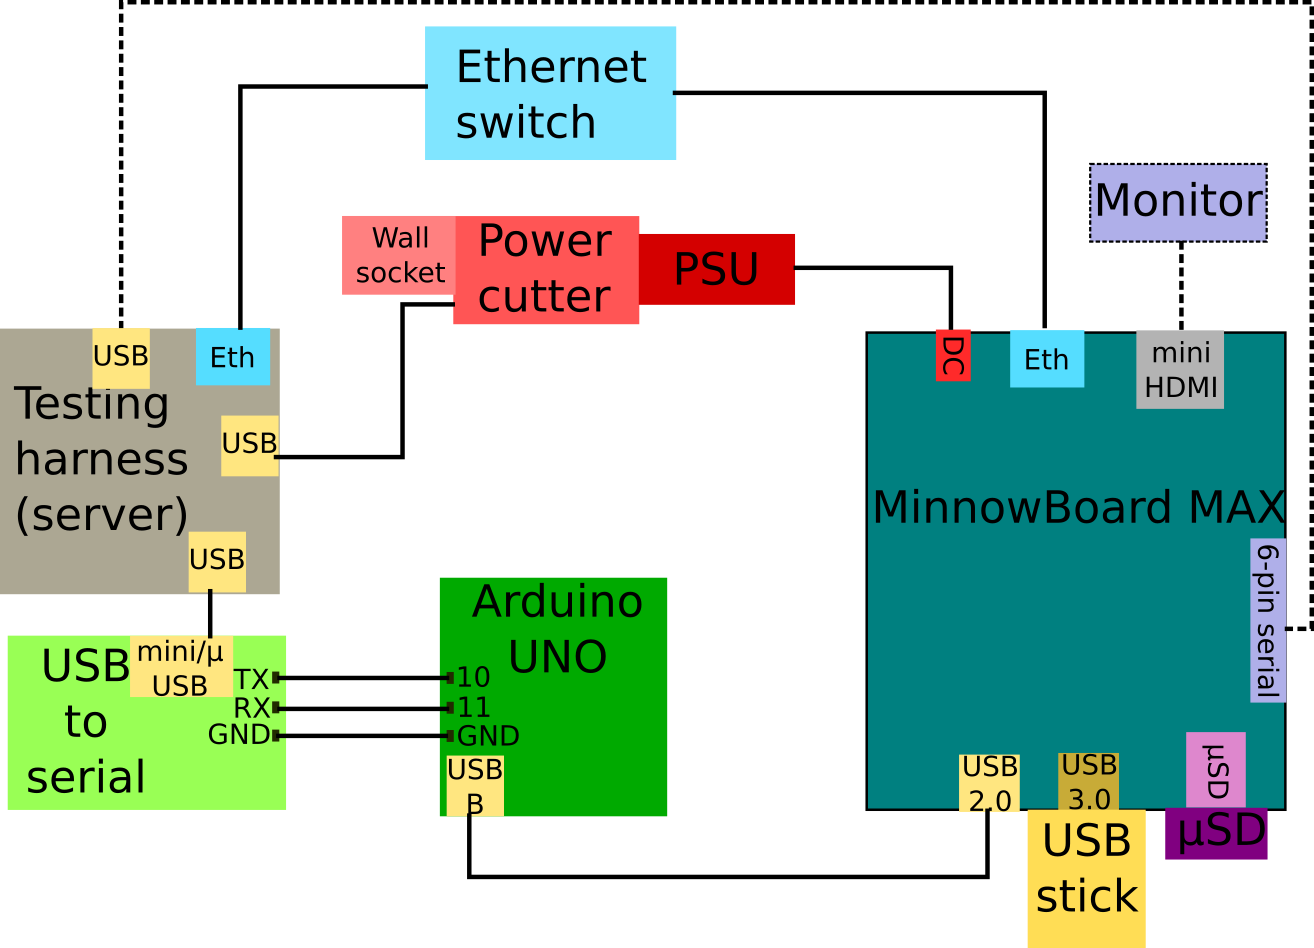
\includegraphics[width=0.7\linewidth]{minnowwiring.png}
	\caption{MinnowBoard MAX wiring diagram}
\end{figure}

\subsection{Simple setup}
The absolutely mandatory steps to take for a simplest working system with just MinnowBoard MAX platform are as follows:
\begin{enumerate}
	\item Copy the content of Testing automation USB-stick from ta-usb-stick branch in the AFT git repository to a suitable USB-stick.

\note{At the time of writing, the location is temporary and doesn't include pre-made Debian images due to their size.}
	\item Setup a Testing harness as instructed in section \ref{testingharness}
	\item Pick a Cleware powercutter and using the instructions on section \ref{clewarecutters}, install the associated software.
	\item Setup AFT as instructed in section \ref{aft}
	\item Setup PEM as instructed in section \ref{pem}
	\item Create an Arduino keyboard emulator using the instructions in \ref{pemarduino}
	\item Using \cmd{dd} create a bootable Debian USB-stick for MinnowBoard MAX as instructed in section \ref{pc}.
	\item Following instructions in the first two subsections of section \ref{minnowboard}, set up the testing hardware.
	\item Configure AFT using the instructions from appendix \ref{app:aft}.
\end{enumerate}

\subsection{Simple device configuration}

Adding devices to the testing setup is a common scenario. This section serves as a tutorial on how to add a Minnowboard MAX to an existing CI setup. The following assumes that the testing harness has already been configured.

Please refer to \ref{app:aft} for a more thorough explanation of the various values seen here (as well as for values used with other devices)

\begin{enumerate}

\item If there are no other PC-like devices such as Galileos in use, we need to modify \cmd{platform.cfg} file under \cmd{/etc/aft/devices/} to add an entry for PC devices.

\begin{lstlisting}
[PC]
leases_file_name = /var/lib/misc/dnsmasq.leases
config_check_keystrokes = /home/tester/kbsequences/empty
\end{lstlisting}

\cmd{leases\_file\_name} contains the path to \cmd{dnsmasq.leases} file. This file is used to determine device IP address.

\cmd{config\_check\_keystrokes} contains the path to the keyboard sequence that will be used during configuration check to verify that the keyboard emulator is functional.

\item If this is the first Minnowboard that is being added, we need to create an entry for Minnowboards in \cmd{catalog.cfg} file under \cmd{/etc/aft/devices/}.

\begin{lstlisting}
[MinnowboardMAX]
platform = PC
cutter_type = ClewareCutter
test_plan = iot_qatest
target_device = /dev/mmcblk0
root_partition = /dev/mmcblk0p2
service_mode = Debian
test_mode = yocto
service_mode_keystrokes = /home/tester/kbsequences/minnowboard/minnowboarddebian
test_mode_keystrokes = /home/tester/kbsequences/empty
serial_bauds = 115200
\end{lstlisting}

The \cmd{platform}-key here points to an existing entry in \cmd{platform.cfg} file. This is case sensitive.

\cmd{cutter\_type} determines the type of the power cutter that will be used. In this particular case, ClewareCutter will be used.

\cmd{test\_plan} determines the test plan manifest that will be used (stored under \cmd{/etc/aft/test\_plan/})

\cmd{target\_device} determines the block device where the testable image will be stored.

\cmd{root\_partition} determines the default root partition that will be used for ssh key injection, if <image-name>-disk-layout.json file has not been provided.

\cmd{service\_mode} defines a string that must be present in \cmd{/proc/version/} of the support image. This is used to check that the device booted into the service mode instead of the test mode.

\cmd{test\_mode} defines a string that works like as described with \cmd{service\_mode}, but successful test mode boot is verified instead.

\cmd{service\_mode\_keystrokes} contains the path to keystroke file that will be used to boot the device into the service mode.

\cmd{test\_mode\_keystrokes} is used as above, but to boot into the test mode instead.

\cmd{serial\_bauds} determines the baud rate of the serial connection.

\item Finally, the device specific details, such as power cutter and serial connection details, need to be added to \cmd{topology.cfg} under \cmd{/etc/aft/devices/}

\begin{lstlisting}

[MINNOWBOARD_1]
model = MinnowboardMAX
id = 00:08:a2:09:ba:01
cutter = 650348
channel = 3
pem_interface = serialconnection
pem_port = /dev/ttyUSB1
serial_port = /dev/ttyUSB0

\end{lstlisting}
The \cmd{model} here points to an entry in \cmd{catalog.cfg}. This is again case sensitive.

The \cmd{id} value must be the device MAC address.

In this particular example, it is assumed that Cleware cutters are being used (as specified in catalog.cfg). \cmd{cutter} and \cmd{channel} values determine the cutter  and the physical socket that will be used.


\cmd{pem\_port} and \cmd{serial\_port} determine the PEM (the keyboard emulator) and serial ports that will be used. Currently the only supported \cmd{pem\_interface} is the \cmd{serialconnection}.

PEM and serial ports can be determined by plugging in the cables and then reading the actual /dev/ttyUSBx entry from \cmd{dmesg}. An example output when plugging in serial cable:

\begin{lstlisting}
[602722.139098] usb 2-1.4.3: new full-speed USB device number 48 using ehci-pci
[602722.238434] usb 2-1.4.3: New USB device found, idVendor=0403, idProduct=6001
[602722.238444] usb 2-1.4.3: New USB device strings: Mfr=1, Product=2, SerialNumber=3
[602722.238450] usb 2-1.4.3: Product: TTL232R-3V3
[602722.238454] usb 2-1.4.3: Manufacturer: FTDI
[602722.238458] usb 2-1.4.3: SerialNumber: FTFRNFUI
[602722.241004] ftdi_sio 2-1.4.3:1.0: FTDI USB Serial Device converter detected
[602722.241089] usb 2-1.4.3: Detected FT232RL
[602722.241718] usb 2-1.4.3: FTDI USB Serial Device converter now attached to ttyUSB0
\end{lstlisting}
In this case, the serial port is /dev/ttyUSB0, as determined by the final line.

The device MAC address can be found by, for example, booting the device once and observing the device MAC address from the \cmd{dnsmasq.conf} file:

\begin{lstlisting}
1469690381 00:08:a2:09:ba:02 192.168.30.144 intel-corei7-64 01:00:08:a2:09:ba:02
\end{lstlisting}

The MAC address in this case is \cmd{00:08:a2:09:ba:02}

\end{enumerate}



\subsection{Testing automation USB-stick}
In this document there are multiple references to a testing automation USB-stick. This stick is intended to contain programs and other tools required for maintaining a complete testing automation system.

\note{At the time of writing, the location is temporary and doesn't include pre-made Debian images due to their size.}

The content can be downloaded from ta-usb-stick branch in the AFT git repository and copied to any suitably large USB-stick.

The content was bundled together during the creation of this document, in December 2015. Therefore the programs may be out of date.

\subsection{SSH-keys}
In the testing automation system SSH-keys are used extensively for authentication. A default SSH-key is included in the testing automation USB-key in folders \cmd{gigabyte} and \cmd{minnowboard}. Additionally, the SSH-key is added to the \cmd{\/root\/.ssh} folder in each pre-made Debian image. \textbf{It is highly recommended that these SSH-keys are replaced with your own ones!} Leaving the default keys in place may expose your system to attacks.

\subsection{Foreword}
This document was originally written by Topi Kuutela over November and December 2015 to relay information regarding testing automation setup in an embedded Linux project. The document was then expanded by Erkka Kääriä to include Beaglebone Black integration. The level of detail is intentionally high to allow the next operator to understand all details of the system. 

This document covers the configuration and construction instructions only for the testing automation part of the continuous integration system used in the project. The testing automation subsystem is not coupled to the build infrastructure other than by the image transmission.

In the first section the configuration and installation of the testing harness, the testing server, is covered. In the second and third sections the usage of the most important pieces of software are detailed. In section 5 the different kinds of power cutter devices are explained and their associated software is explained. In sections 6-10 the individual testing platforms are described. Finally, in the appendices, the AFT implementation details and privilege reduction options are explained.

\section{Testing harness}
\label{testingharness}
The testing server is, in this document, called testing harness. The testing harness is responsible of fetching the images from the source and executing AFT to flash the images on various target devices. The system has been tested using \emph{OpenSUSE 13.2}.

The testing harness acts to the testable devices as a network file system server, and as a DHCP-server. It is highly recommended that the devices are put in an isolated network.

Testable images can be copied from the builders using many means. Both NFS and standard IP transmission using \cmd{wget} have been tested and found reliable. Because the images are most likely copied over Ethernet, and the testable devices are in a separate network, the testing harness must have two network cards.

In the following section the configuration is detailed. The commands are expected to be run using \cmd{root} privileges. A fresh installation of OpenSUSE 13.2 with SSH-server, no desktop environment and working internet connectivity are assumed. Firewall configuration is not provided, it is recommended that the testing harness is only kept in a trusted network.

Configuration of AFT is explained in appendix \ref{app:aft}.

\subsection*{Base system}
A set of common tools and utilities:
\begin{lstlisting}
zypper install git gcc gcc-c++ make automake cmake autoconf man emacs nano screen tree attr dnsmasq gdisk nfs-kernel-server python python-setuptools python-devel python-tk python-idle ipython libusb-1_0-devel usbutils tftp yast2-tftp-server guestfs-tools
\end{lstlisting}


OpenSUSE comes with \cmd{YaST} configuration utility. It can be used to configure most base OS options. Using \cmd{yast} configure:
\begin{enumerate}
\item The secondary Ethernet card to have static IP \cmd{192.168.30.1}, and subnet mask \cmd{255.255.255.0}
\item Create user \cmd{tester} and add it to \cmd{wheel} group
\end{enumerate}
The secondary local area network is used for the flashing of PC-devices  \ref{pc} and Beaglebones \ref{bbb}. The \cmd{tester}'s  home will be set as shared folder over NFS for the \cmd{192.168.30.0/24} network. The \cmd{tester} is also the recommended user for automated testing.

Enable \cmd{wheel} group as passwordless sudoers. Using \cmd{visudo} add to the end of the \cmd{/etc/sudoers} file:
\begin{lstlisting}
%wheel	ALL=(ALL)	NOPASSWD: ALL
\end{lstlisting}

\subsection*{DFU-util}
\label{dfuutil}

Flashing Edison requires the installation of \cmd{dfu-util} program. Dfu-util takes care of the DFU-protocol and the flashing of each partition on the target device.

In order to support multiple Edisons, dfu-util requires USB-tree support. Fortunately this support was recently (at the time of writing, 17.2.2016) merged to the codebase. When installing dfu-util, make sure that the installed version contains this patch. 

Dfu-util can also be built from the source, using the following steps.

\note See \ref{gitclone} if git clone fails

\begin{lstlisting}
git clone git://git.code.sf.net/p/dfu-util/dfu-util dfu-util-src
cd dfu-util-src
./autogen
./configure
make
make install
\end{lstlisting}

The USB-tree patch is available at \\ \cmd{http://sourceforge.net/p/dfu-util/tickets/6/attachment/0001-Fix-reimplement-\\USBPATH-support.patch} if it is required.

\subsection*{Edison recovery tool}

Edison recovery flashing requires a tool that is not available in the regular repositories. It can be installed by adding \\
\cmd{http://download.opensuse.org/repositories/home:/lvader:/xfstk/
openSUSE\_13.2/} \\
to the available repositories by using \cmd{YaST} (Software -> Software repositories -> Add). The tool can then be installed with zypper:
\begin{lstlisting}
zypper install xfstk-downloader-solo
\end{lstlisting}

\subsection*{Git proxy}
\label{gitclone}
If \cmd{git clone} fails (time outs or gets stuck), a proxy script may be needed for \cmd{git clone} to work.

Begin by installing socat

\begin{lstlisting}
zypper install socat
\end{lstlisting}

Then create \cmd{git-proxy} under \cmd{/usr/bin} and add the the following lines into this file

\begin{lstlisting}
#!/bin/bash
# $1 = hostname, $2 = port
PROXY=proxy.server.address.here.com
exec socat STDIO SOCKS4:$PROXY:$1:$2
\end{lstlisting}

Where \cmd{PROXY} must be appropriately
The file needs to be executable

\begin{lstlisting}
chmod +x /usr/bin/git-proxy
\end{lstlisting}

Finally add the following lines under your .gitconfig file (\cmd{\textasciitilde/.gitconfig})

\begin{lstlisting}
[core]
	gitproxy=git-proxy
\end{lstlisting}

\subsection*{Clewarecontrol}
Clewarecontrol utility is used to control the power cutters made by Cleware GmbH. At the time of writing, the latest clewarecontrol, version 4.1, was broken. Therefore the version 2.8 is recommended.

To install clewarecontrol commandline utility:
\begin{lstlisting}
wget https://www.vanheusden.com/clewarecontrol/files/clewarecontrol-2.8.tgz
tar -xvf clewarecontrol-2.8.tgz
cd clewarecontrol-2.8
make
make install
\end{lstlisting}

Usage instructions are given in the section \ref{powercutters}.

\subsection*{Dnsmasq}
\cmd{Dnsmasq} is used as a DHCP-server for the PC-devices. It also provides a table with MAC-to-IP-address conversion. Dnsmasq is configured to provide IP-addresses to the \cmd{192.168.30.0/24} subnet, to all devices connected (through a switch) to the secondary Ethernet port.

Add the following lines to \cmd{/etc/dnsmasq.conf} file:
\begin{lstlisting}
dhcp-range=192.168.30.2,192.168.30.254,10m
interface=p1p1
\end{lstlisting}
\note{replace the \cmd{p1p1} with the network interface the PC-devices are connected to.}

To enable dnsmasq service:
\begin{lstlisting}
systemctl start dnsmasq.service
systemctl enable dnsmasq.service
\end{lstlisting}
If at some point the DHCP-exchange has to be debugged, stop the Systemd-service and start dnsmasq manually using:
\begin{lstlisting}
systemctl stop dnsmasq.service
dnsmasq --no-daemon
\end{lstlisting}

The dnsmasq IP leases can be found (by default) from \cmd{/var/lib/misc/dnsmasq.leases}

\subsection*{Network File System}
Network file system (NFS) is used to share the images and other files used in flashing for PC-devices. By convention the whole \cmd{/home/tester} is shared.

To share the folder, add the following line to \cmd{/etc/exports}:
\begin{lstlisting}
/home/tester 192.168.0.0/16(crossmnt,ro,root_squash,sync,no_subtree_check)
\end{lstlisting}

Then enable the Systemd-service:
\begin{lstlisting}
systemctl start nfs-server.service
systemctl enable nfs-server.service
\end{lstlisting}
On some platforms, also \cmd{rpcbind.service} has to be activated.

\subsection*{TFTP-server}

Beaglebone Black uses its support image over NFS. However, it downloads the initial kernel image and device tree binaries using TFTP protocol.

TFTP server can be configured easily with YAST.

\begin{lstlisting}
Start YAST
Open Network Services menu
Select TFTP server
Enable the server
Set Boot Image Directory as /home/tester/
\end{lstlisting}

\note The above assumes that the tests are run under tester-user, and that the default AFT \ref{aft} settings for Beaglebone are used. Adjust the Boot Image Directory if needed. The path should be the same than the nfs folder on the testing harness.

\subsection*{Udev (optional)}
It is recommended to set udev-rules to create symbolic links from a human-readable file name to ttyUSB-devices used for PEM (section \ref{pem}), serial output recording (appendix \ref{app:aft}) and to the USB-relay powercutters used for Edisons. The USB-to-serial adapters are often unreliable and tend to occasionally reset, which causes a re-initialization by Linux kernel. This also triggers a (re-)creation of the ttyUSB-device created by udev.

The recommended way to set the rules is by adding rules to, for example, \\ \cmd{/etc/udev/rules.d/99-persistent-ttyusb}. A rule can look for example like:
\begin{lstlisting}
SUBSYSTEM=="tty", ENV{ID_PATH}=="pci-0000:00:1d.7-usb-0:1.1.3:1.0", SYMLINK+="gigabytearduino3"
\end{lstlisting}
The \cmd{SUBSYSTEM} is the udev subsystem which is used by the target device, the \cmd{SYMLINK} is the name of the symbolic link created under \cmd{/dev}, and the \cmd{ID\_PATH} is used to filter the specific device. To retrieve the {ID\_PATH}, plug in the device, find the correct \cmd{ttyUSBX} device using e.g. \cmd{dmesg} and execute:
\begin{lstlisting}
udevadm info /dev/ttyUSBX
\end{lstlisting}

After setting the rules, udev must be refreshed using
\begin{lstlisting}
udevadm trigger
\end{lstlisting}

\note Setting the rules using this method allows unplugging and re-plugging USB-cables to the same port, or rebooting the testing harness without re-configuring AFT. Otherwise the ttyUSB-device may change!

\section{AFT - Automated Flasher Tester}
\label{aft}

AFT is a Python tool to flash the testable image to various kinds of devices.  AFT tries to guarantee that the device under test is in a state where:
\begin{itemize}
\item The device can be rebooted and the image under test starts again.
\item The device under test can be accessed over SSH without a password.
\end{itemize}

To achieve the first requirement, AFT flashes the image to the primary boot media of the device under test, and possibly modifies the BIOS settings to use that as the boot media.

The second requirement is achieved by injecting a known public SSH-key to \linebreak\cmd{<root home>/.ssh/authorized\_keys}. This allows the owner of the corresponding private key to connect the device without a password. AFT may also modify the network settings of the testing harness to make sure the device is still accessible after a reboot.

Finally AFT starts the pre-configured tests by executing either its internal test cases or by starting a subprocess. The test cases are assumed not to modify the BIOS settings. For this AFT has an integrated test runner which executes test plans based on configuration.

Because flashing often requires multiple boots during the process, and the only guaranteed way to power off a device is to cut its power, different kinds of external power cutters are used.

The execution syntax for AFT is
\begin{lstlisting}
aft <machinetype> <imagefile>
\end{lstlisting}
where, at the time of writing, the options for  \cmd{machinetype} are \cmd{gigabyte}, \cmd{galileov2}, \cmd{minnowboardmax}, \cmd{edison} and \cmd{beagleboneblack}. The imagefile is the image to be tested, with the exception of Beaglebone Black, where the argument is (mis)used to provide path to the directory with all the files that are required for flashing. It is recommended to use the current working directory for this, which allows using \cmd{`pwd`} as the parameter.

Optionally, AFT can also record the serial console output to file by using \cmd{-\/-record} argument, assuming the serial device has been configured properly. This allows some level of logging even if the device fails to boot.

Details to the configuration of AFT is given in the appendix \ref{app:aft}. In the same appendix there is a a general overview to the classes involved and implementation details.

\subsection{PC-devices}
\label{pc}
PC-like devices are devices which have a network interface with a fixed MAC-address and usually have a some sort of BIOS/EFI menu.

PC-like devices are flashed with the aid of a \textit{support image}, a Linux image which can boot the device under test. The support image is used to copy the target image over NFS to the primary boot media, and to add e.g. the SSH-key to it.

The BIOS settings are modified using PEM, an Arduino UNO device with a keyboard emulating firmware. See section \ref{pem} for further information.

The biggest hurdle with PC-devices is usually the creation of a support image. The distribution used on this guide is Debian 8.2 because it supports out of the box a wide range of architectures and is generally known to be compatible with many kinds of devices. In simple cases the support image creation is just a matter of installing the operating system to a USB stick. In worse cases, e.g. with Galileo Gen 2, it requires the creation of custom kernel with board specific \textit{Board Support Package} (BSP).

Support images for all currently supported devices are provided on the testing automation USB-stick.

By using a support image to also modify the target image, AFT can be run without root privileges. \cmd{Mount}-command for modifying images and mount points always requires root privileges, but this is executed only on the support image. Unfortunately gadget-devices require the modification of the image on the testing harness, so this is not viable in the general case.

PC-devices usually use some kind of a power supply which is connected to the mains powerlines. Therefore a natural place for a power cutter is in between the mains and the PSU.

Another option would be to strip the positive line between the PSU and the device, and install a power cutter in between. This is considered a worse solution because it requires more customization of the hardware.

The PC-devices described in this document include Gigabyte \ref{gigabyte}, MinnowBoard MAX \ref{minnowboard} and Galileo Gen 2 \ref{galileo}. 

A support image is provided on the Testing automation USB-stick for each platform in the folder \cmd{debian-images}. These can be copied to another USB-stick using e.g.
\begin{lstlisting}
dd if=<USB-root>/debian-images/minnowUSB.image of=/dev/sdX bs=8M
\end{lstlisting}
where the \cmd{sdX} refers to the block device you want to copy the image to.

\subsection{Gadget-devices}

Gadget-like devices are devices which are closer to a mobile phone or a traditional embedded MCU or SoC. These are often flashed using the DFU-protocol.

There are several DFU programmer utilities and flashing a device completely may require separate flashing calls to flash each memory media on the device. Depending on the flashing utility, it may be possible to detect errors during flashing. These shouldn't cause a failure in testing but instead just initiate another attempt at flashing.

Depending on the device, switching power on and off can be considerably more difficult with a gadget-device. If the testable device has an internal battery, it most likely requires somewhat complicated custom hardware to power cycle it. With gadget-devices extra care must be taken in the prevention of floating ground issues. If the device is powered over USB, a powered USB-hub is almost certainly required.

The only gadget-device in this document is the Intel Edison \ref{edison}, which uses dfu-util (\ref{dfuutil}) for flashing and a USB-relay as a power cutter.

\subsection{Beaglebone Black}
\label{bbb}

For the purposes of the document, Beaglebone Black is a hybrid gadget/PC device. It is an ARM device, it does not have a BIOS and it uses u-boot as its bootloader. However like PC devices, it requires support image to bypass its unfortunate flashing protocol which requires manual steps from the operator. 

\section{PEM - Peripheral EMulator}
\label{pem}

\note{The instructions work only on Arduino UNO!}

Peripheral Emulator is a device created out of an Arduino UNO and USB-to-serial adapter for emulating a keyboard or another peripheral device. To be compatible with the PC 97 standard, and especially BIOS mode, the firmware supports 6-key-rollover.

PEM works by flashing both the Atmega 328U and Atmega 16U2 chips on the Arduino UNO R3 board. 

The Atmega 328U is flashed with a firmware that takes care of the communication between the testing harness and the USB-to-serial adapter. The firmware receives keyboard states from the testing harness over serial data line and responds with an acknowledgement after each successful packet.

The Atmega 16U2 is converted from its original USB-to-serial mode to an actual 6KRO HID-emulator. The 16U2 receives the packets from the 328U, interprets them and sends them over the USB-interface using HID protocol.

PEM can be installed by issuing the following commands:
\begin{lstlisting}
git clone https://github.com/01org-AutomatedFlasherTester/pem.git
cd pem
sudo python setup.py install
\end{lstlisting}
\note{PEM installation files are also included in the Testing automation USB-stick in the \cmd{installationfiles} folder.}

\subsection{Creation of a PEM-Arduino}
\label{pemarduino}
The creation of a PEM-Arduino requires 
\begin{itemize}
\item An Arduino UNO R3
\item USB-to-serial adapter
\item 3 wires to connect the USB-to-serial adapter to Arduino
\item A jumper or a piece of wire
\item USB A to USB B cable
\item USB A to mini/microUSB (depending on the USB-to-serial adapter)
\end{itemize}

The programs required are the Arduino IDE 1.6: (\url{https://www.arduino.cc/en/Main/Software}) and dfu-programmer 0.62: (\url{https://dfu-programmer.github.io/}).

\begin{enumerate}
\item Plug the Arduino UNO to your computer using the USB-B to USB-A connector.

\item Start the Arduino IDE. Select the correct port in the \cmd{Tools->Port} menu. Open the \cmd{<PEM git repository>/src/pem\_Arduino/pem\_Arduino.ino}. Flash the sketch in the Arduino. Close the IDE.

\item With the Arduino connected to computer (and powered), connect briefly using a jumper or a piece of wire the two pins closest to the Arduino's USB-B port. This resets the Atmega 16U2. Now you should be able to get (scrambled) output by issuing:
\begin{lstlisting}
sudo dfu-programmer atmega16u2 dump
\end{lstlisting}

\item The firmware for the 16U2 is included in the testing automation USB-stick but it can also be downloaded from \url{http://hunt.net.nz/users/darran/weblog/b3029/Arduino_UNO_Keyboard_HID_version_03.html}. To flash the firmware, in the testing automation USB stick folder \cmd{arduinokb}, issue the following command:
\begin{lstlisting}
sudo sh flash.sh
\end{lstlisting}
This script first erases the 16U2, then flashes the firmware and then resets the chip.

\item To verify that the system works, see the usage instructions in the following subsection.
\end{enumerate}

\subsection{Usage instructions}
PEM has a graphical user interface for recording keyboard sequences. To make the keyboard sequence as reliable as possible, it is good idea to use constant intervals between the key presses. Additionally, most BIOS menus support e.g. PageUp and PageDown keys which move the cursor to the top or the bottom of the list (that is, to a known, fixed location).

When using the peripheral emulator, connect the USB-to-serial to your testing harness or recording computer using the mini/microUSB connector. Connect the USB-to-serial pins to corresponding Arduino pins: \cmd{TX => 10}, \cmd{RX => 11} and \cmd{GND => GND}.

When PEM is started, it doesn't start sending the key presses before the target device can detect them. This is achieved by waiting for the Arduino to boot up. Arduino is powered by the USB-B line, and therefore gets the power when the target device boots. Because the device under test power is controlled using a mains power cutter, in production, the PEM starts sending the key presses only exactly when the device boots.

To start the recording interface, use
\begin{lstlisting}
sudo pem --interface serialconnection --record <target_file> --port </dev/ttyUSBX>
\end{lstlisting}
\note replace the \cmd{/dev/ttyUSBX} with the \cmd{ttyUSB}-device corresponding to the USB-to-serial adapter, which can be found using e.g. \cmd{dmesg}.

In the recording interface, to start recording a sequence, press the \cmd{Start} button. After that, each key press sent to the PEM UI gets sent to the target device. To stop recording and to save the last recording to the file given in the command line arguments, press the  \cmd{Stop} button.

To clean up the keyboard sequence, a LibreOffice Calc spreadsheet is provided on the testing automation USB-stick at \cmd{<USB-root>/arduinokb/sequence-editor.ods}.

To execute a keyboard sequence, use the following command
\begin{lstlisting}
sudo pem --interface serialconnection --playback <playback_file> --port </dev/ttyUSBX>
\end{lstlisting}

\section{Power cutters}
\label{powercutters}
Controlling the power on the target devices is always done using a power cutter in the power line. Power cutters are used because powering off cleanly is not reliable. In some PC-devices, the USB-ports also remain powered unless the power is completely cut off.

\subsection{Cleware powercutters}
\label{clewarecutters}
In our setup we have used two kinds of power cutters: for PC-devices, power switches by Cleware GmbH are used. Cleware cutters are controlled over USB using a command line tool \cmd{clewarecontrol}. At the time of writing, the latest version of \cmd{clewarecontrol}, 4.1, is unstable at least on Linux Fedora 22. It is recommended to use the version 2.8.

The cutters can be listed by issuing
\begin{lstlisting}
clewarecontrol -l
\end{lstlisting}

A switch can be turned on and off using the following command
\begin{lstlisting}
clewarecontrol -d <device ID> -c 1 -as X [1|0]
\end{lstlisting}
where device ID is the ID of the cutter device, \cmd{X} is the index of power socket in the cutter (zero-based), and the last number is 1 for switching the socket on, and 0 for switching it off.

\subsection{USB-relays}
The Edison is controlled using a USB-relay in the +5V line on the USB-cable. The relay is controlled using a Python script shipped with the AFT. The script sends binary data over serial to switch the relay on and off.

The USB-relays can be ordered from e.g. eBay. In some cases the switches are incorrectly recognized by the testing harness. The serial controller identifies itself as something else but a USB-to-serial adapter. The cause is probably incorrect internal firmware.

This can be fixed by adding a custom USB device ID to the correct USB-to-serial driver. The driver depends on the USB-to-serial chip used in the relay, common ones being \cmd{cp210x} and \cmd{ftdi\_sio}. Adding a new device can be done in a root terminal by using for example
\begin{lstlisting}
echo "0b00 3070" > /sys/bus/usb-serial/drivers/cp210x/new_id
\end{lstlisting}
The device ID can be found with the help of e.g. \cmd{lsusb}. If the driver is not loaded, it can be loaded manually using \cmd{modprobe}.

\section{Gigabyte GB-BXBT-3825}
\label{gigabyte}

Gigabyte is an IoT-gateway platform. It has a Gigabit ethernet, two USB 2.0 ports and one USB 3.0 port, HDMI- and VGA-outputs and internal WLAN and Bluetooth cards. It comes with 2 GB of ram and Intel Atom E3825 - the same one as in MinnowBoard MAX. It also has a 500 GB internal hard drive, which is the boot device used for testing.

The BIOS of Gigabyte has basic settings for boot option priorities and overriding the boot priorities. It also has options to restart the device on AC power loss, which has to be set as the booting is executed using a powercutter. Gigabyte supports Secure boot, but also has options for disabling it and to let users add their own keys. To enter the BIOS press delete-key during boot.

\note the BIOS only supports one boot media with legacy boot (MBR), which must be set as the \cmd{Boot Option \#1} in \cmd{Boot => Hard Drive BBS Priorities}.

\note the USB 3.0 port in the front of the device doesn't work as a boot device if used with a USB 3.0 stick.

\note Gigabyte BIOS is notoriously buggy. It sometimes creates invisible options to the boot override menu which replace a valid option but don't work. To fix this, reflash the BIOS.

\note At the time of writing, Gigabyte requires a screen attached to the HDMI port in order to boot in MBR mode. A screen in the VGA port does not work.

Gigabyte supports only 12V DC input and requires a 2.5 A powersupply. The DC-plug has a positive center.

\subsection{CI-integration}
Gigabyte is a PC-like device, similar to Galileo Gen 2 and MinnowBoard MAX. A Debian support image is created on a USB-stick. It is recommended that the support image is created with a legacy (non-EFI) bootloader. The BIOS settings are controlled with PEM-Arduino. The internal hard drive is used for the target image.

The internal ethernet adapter is used for networking.

The PEM keyboard sequence should select the support image from \cmd{Save \& Exit => Boot Override} menu. The image boot options should (automatically) be the top options in the boot option priorities so the keyboard sequence for testing should be empty.

\begin{figure}[h]
	\centering
	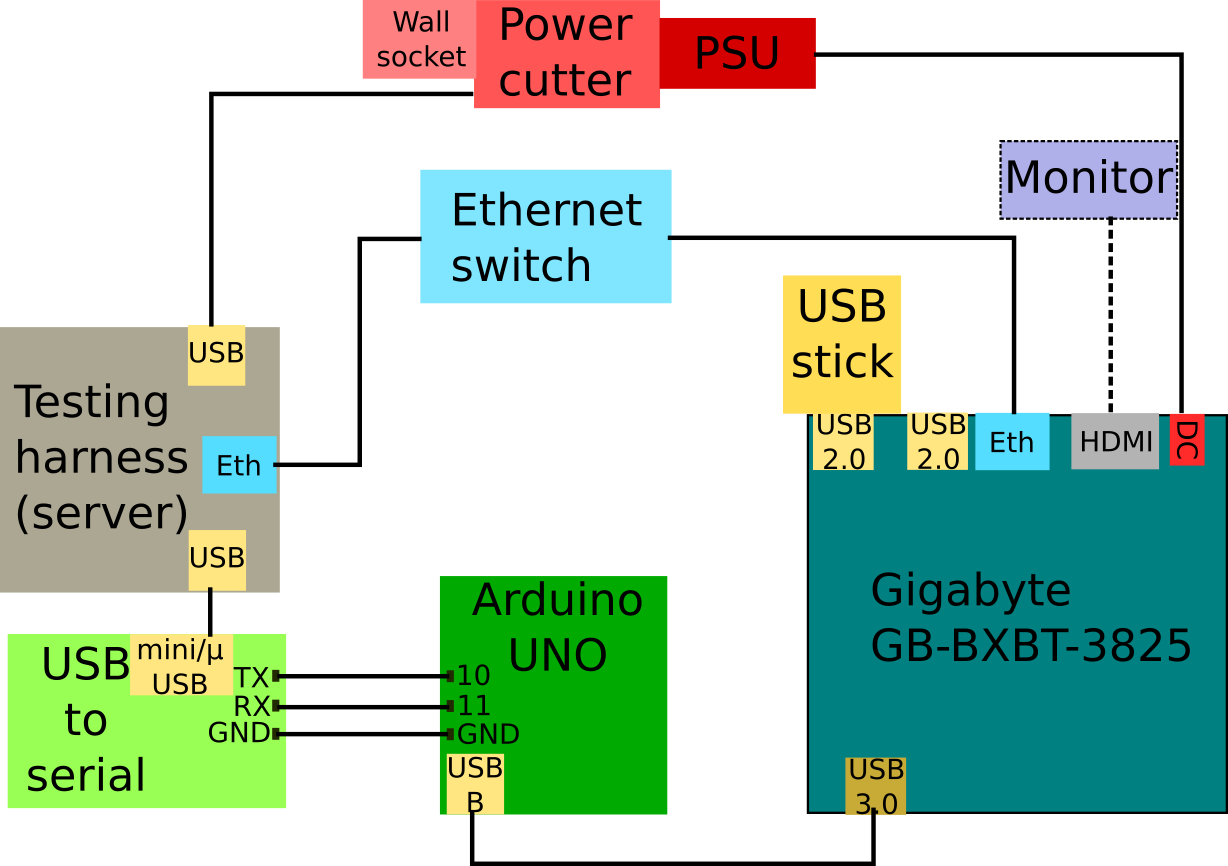
\includegraphics[width=0.7\linewidth]{gigabytewiring.png}
	\caption{Gigabyte GB-BXBT-3825 wiring diagram}
	\label{fig:gigabytewiring}
\end{figure}

\subsection{Debian on Gigabyte}
These instructions are for creating a bootable Debian USB-stick for Gigabyte with MBR and persistent storage.

\begin{enumerate}
\item Make sure the internal hard drive doesn't have a bootloader, or nuke the hard drive: 

\item Update the BIOS


\begin{lstlisting}
dd if=/dev/zero of=/dev/sda bs=8M count=500
\end{lstlisting}

\item In the BIOS disable Secure boot and set the

\cmd{Chipset => Restore AC Power Loss} to \cmd{Power On}.

\item Dd a 64-bit Debian installation DVD to USB-stick:


\begin{lstlisting}
dd if=debian-8.2.0-amd64-DVD-1.iso of=/dev/sdX bs=8M; sync
\end{lstlisting}

\item Plug the USB-stick on a USB 2.0 port, boot the device and enter BIOS. \note if the USB-stick is a USB 3.0 stick, it will not boot from the USB 3.0 port!

\item Select the USB-stick as the primary legacy boot option in \cmd{Boot => Hard Drive BBS Priorities}. Select the USB-stick as the boot override option in \cmd{Save \& Exit => Boot Override}.

\item Only plug the target USB-stick after Debian installer menu is visible.

\item Start Debian installation.

\item When prompted for missing firmware files, don't try to install them at this phase (answer 'no').

\item Select hostname, use e.g. Debian-gigabyte.

\item Root password: \cmd{rootme}

\item User name: \cmd{user}, real name: \cmd{user}, password: \cmd{user}.

\item For partitioning, automatical partition for entire disk with all files in one partition works. Remember to select the correct USB-drive.

\item When prompted for software selection, the spacebar enables and disables options. Disable Debian desktop environment and print server, but enable SSH server. Enter to continue.

\item Once the installation is finished, remove the installation media, set the remaining USB-stick as the primary legacy boot option and boot the newly installed Debian.

\item Once booted, log in as \cmd{root}, plug in the test automation USB-stick and execute:

\begin{lstlisting}
mkdir temp; mount /dev/sdc1 temp; cd temp/gigabyte; ./installgigabyte; cd; umount temp; rm -r temp
\end{lstlisting}

See the comments on the test automation USB-stick \cmd{gigabyte/installgigabyte} script for details of the post installation configuration.

\item Reboot the device and from the BIOS menu, boot the Debian image.

\item Manually flash the internal hard drive with a current testable image.

\item Reboot the device, adjust the boot priorities so that the primary options are from the testable image.
\end{enumerate}

\subsection{Flashing the BIOS on Gigabyte}
Out of the box, Gigabyte comes with a 32-bit BIOS. This means that the EFI-stub also has to be 32-bit (which, still, can load a 64-bit OS). This can be fixed by updating the BIOS to a 64-bit version, which is supplied by Intel.

The testing automation USB-stick contains all the files required to update the BIOS to version \cmd{F2a x64} in the folder gigabytebios. The official instructions are available at \url{https://wiki.ith.intel.com/display/TME/ODM+Gateway+BIOS+Files}.

The following instructions assume that you have copied the latest version to the USB-stick.

\begin{enumerate}

\item Plug the USB-stick to the Gigabyte. Reboot the device, enter BIOS and set the first boot device to UEFI: Built-in EFI Shell.

\item In EFI Shell, first select the correct device from the Device mapping table. The most likely candidate for the USB-key is \cmd{fs0}:
\begin{lstlisting}
fs0:
\end{lstlisting}
\note the keyboard uses the US-layout.

\item go to the \cmd{gigabytebios} folder:

\begin{lstlisting}
cd gigabytebios
\end{lstlisting}

\item Execute the flashing. If the \textit{current} BIOS is 32-bit use \cmd{fpt}, or if the current BIOS is 64-bit use \cmd{fpt64}.

\begin{lstlisting}
fpt64 -f BAYADx64.F2a
\end{lstlisting}

\item After the flashing is completed, reboot the device by issuing:
\begin{lstlisting}
reset
\end{lstlisting}
\note flashing the BIOS resets the BIOS settings. Remember to disable secure boot and set the device to power on after AC power loss.

\end{enumerate}


\section{MinnowBoard MAX and MinnowBoard Turbot}
\label{minnowboard}

MinnowBoard MAX is an open development board with a 64-bit Intel Atom E3825 CPU (the same as in Gigabyte) and 2 GB ram. It provides one microSD slot, a SATA2 connector, one of each USB 2.0 and USB 3.0 sockets, gigabit ethernet and a 6-pin serial output. It also has a microHDMI connector for monitors.

MinnowBoard Turbot is a MinnowBoard Max-compatible derivative board. It fixes several hardware related issues and uses a slightly faster Intel Atom E3826 CPU. For the purpose of this documentation, Turbot is interchangeable with Max (\note: Turbot is also compatible with MAX BIOSes).

MinnowBoard MAX uses EFI for hardware initialization. The BIOS menu can be entered by pressing \cmd{F2} during boot. The boot priorities can be overridden in the \cmd{Boot Manager} menu, and the priorities can be adjusted in \cmd{Boot Maintenance Manager}.

\subsection{CI-integration}

\begin{figure}[h]
	\centering
	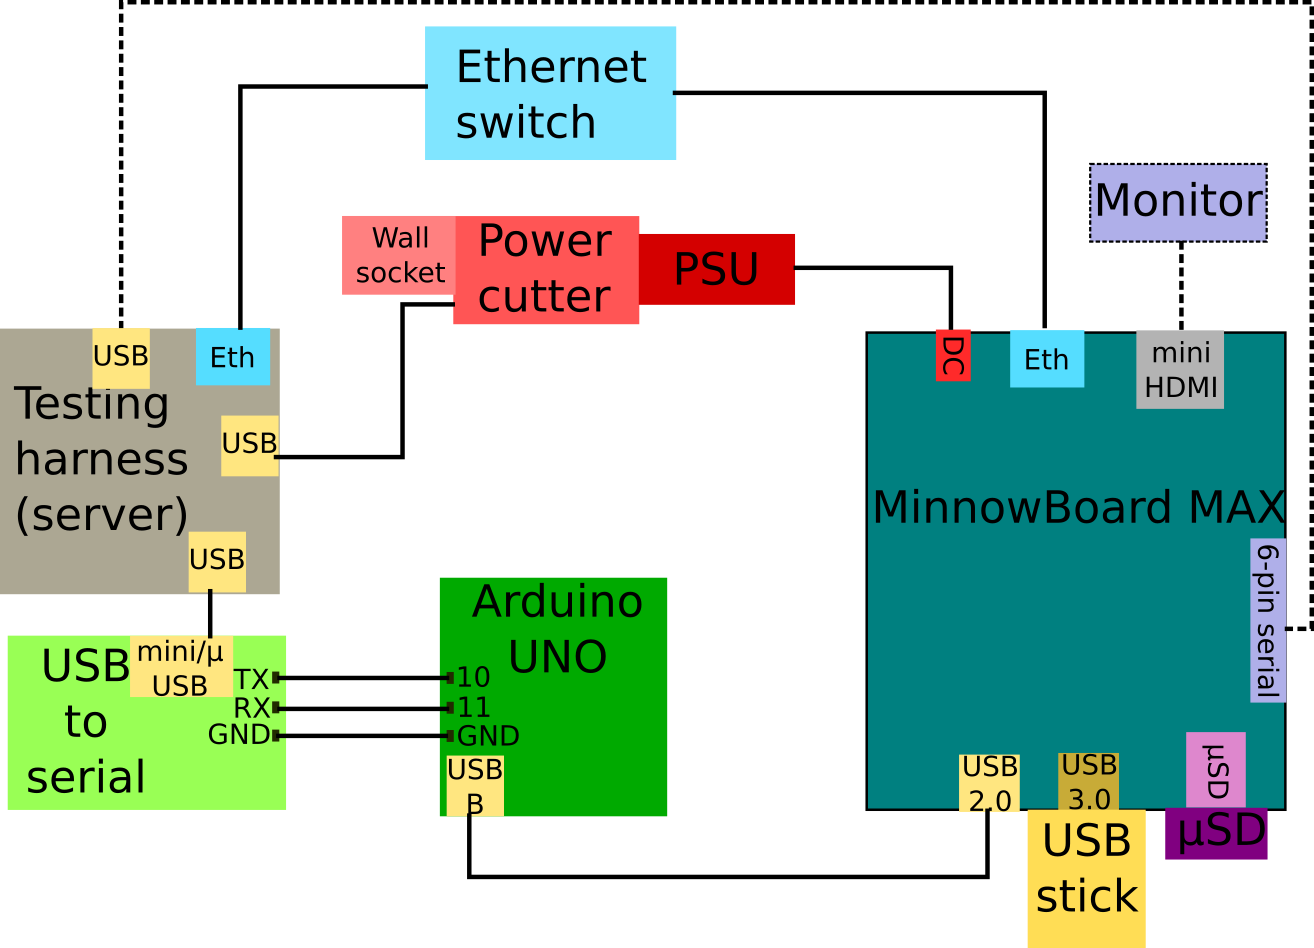
\includegraphics[width=0.7\linewidth]{minnowwiring.png}
	\caption{MinnowBoard MAX wiring diagram}
	\label{fig:minnowwiring}
\end{figure}

MinnowBoard MAX is a PC-like device, similar to Gigabyte and Galileo Gen 2. A Debian support image is created on a USB-stick. For MinnowBoard MAX Debian, an EFI-enabled bootloader is used but it has to be slightly modified for more convenient and stable test automation. The instructions for this are at the end of section \ref{minnowdebian}.

The internal ethernet adapter is used for network connectivity.

After the bootloader modification, the PEM keyboard sequence can be used to select \cmd{EFI USB Device} as the boot device in the \cmd{Boot Manager} menu. The boot partitions of the image under test should be set as the primary boot options in the \cmd{Boot Maintenance Manager} so that an empty keyboard sequence can be used to boot it.

The 6-pin serial output can be used for boot console recording at 115200 bauds.

The microSD-card is used for the target image with MinnowBoard MAX.

\subsection{Flashing the BIOS on MinnowBoard MAX}

MinnowBoard MAX supports both 32- and 64-bit firmwares. The official firmware site is \url{https://firmware.intel.com/projects/minnowboard-max} but the firmware version \cmd{0.83} has been added to the testing automation USB-stick with both 32- and 64-bit flashing utilities. The following instructions explain how to flash the firmware using the testing automation USB-stick.

\begin{enumerate}
\item Attach the testing automation USB-stick to MinnowBoard MAX along with a keyboard and a monitor.

\item Reboot the device and enter the BIOS menu. Determine the architecture of current BIOS from the third line in the header. For example, \textit{MNW2MAX1.\textbf{X64}.0083.R01.1509181113}.

\item Select \cmd{EFI Internal Shell} as the boot media. (\cmd{Boot Manager => EFI Internal Shell}).

\item Enter the USB-stick file system with the help of \cmd{Mapping Table}. In this example the USB-stick has been mapped to \cmd{FS0}. Note that the keyboard layout is US.
\begin{lstlisting}
FS0:
\end{lstlisting}

\item Change to the \cmd{minnowboardbios} folder:
\begin{lstlisting}
cd minnowboardbios
\end{lstlisting}

\item Based on the BIOS version architecture, execute the correct updater; for X64 system \cmd{MinnowBoard.MAX.FirmwareUpdateX64.efi} and for IA32 systems the IA32 version.
\begin{lstlisting}
MinnowBoard.MAX.FirmwareUpdateX64.efi MinnowBoard.MAX.X64.083.R01.bin
\end{lstlisting}

\item The system will shut down after flashing is complete. You will have to reconfigure the BIOS settings after the update.
\end{enumerate}

\subsection{Debian on MinnowBoard MAX}
\label{minnowdebian}

Because MinnowBoard MAX has only two USB-ports, and one of them is required for a keyboard, a microSD-card must be used for installation media. The BIOS doesn't support USB hubs but they can be used after the OS is booted.

\begin{enumerate}
\item Flash a 64-bit Debian installation image on a microSD-card:

\begin{lstlisting}
dd if=debian-8.2.0-amd64-DVD-1.iso of=/dev/sdX bs=8M; sync
\end{lstlisting}
Select \cmd{X} to match the SD-card device on your machine with the help of e.g. \cmd{lsblk}.

\item Using e.g. \cmd{gparted} remove the default partitioning of the target USB-stick.

\item Insert the SD-card to a MinnowBoard MAX. Do \emph{not} insert the USB stick yet!. Reboot the device and from BIOS menu select the Misc device to boot from the SD-card. A Debian installer menu should appear.

\item Insert the target USB-stick.

\item Start installation, select language (English), locale (Irish) and keyboard layout (Finnish).

\item When prompted for CD-ROM drivers, select \cmd{No}. Then manually select the CD-ROM module and device (\cmd{yes}), select the module needed for access the CD-ROM (\cmd{none}) and device file for accessing the CD-ROM: \cmd{/dev/mmcblk0}.

\item When prompted for missing firmware files, don't try to install them at this point (answer: No).

\item Select hostname, use e.g. Debian-MinnowMAX, and leave the network name empty.

\item Set the root password, use \cmd{rootme}

\item Create a user, use user name: \cmd{user}, real name: \cmd{user} and password \cmd{user}.

\item Adding a network package source is not necessary, it is added by a post-install script.

\item When prompted for software selection, the spacebar enables and disables options. Disable Debian desktop environment and print server, but enable SSH server. Enter to continue.

\item After the installation is finished, eject the microSD-card, select \cmd{debian} as the boot device in the BIOS \cmd{Boot Manager} and login to the Debian.

\item Format the microSD-card and from the testing automation USB-stick, copy the contents of the contents of \cmd{minnowboard} folder to the card.

\item Plug the SD-card in the MinnowBoard MAX, execute the following:
\begin{lstlisting}
cd; mkdir temp; mount /dev/mmcblk0p1 templs; cd temp; chmod +x installminnow; ./installminnow; cd; umount /dev/mmcblk0p1; rm -r temp
\end{lstlisting}

See the comments on the test automation USB-stick \cmd{minnowboard/installminnow} script for details of the post installation configuration.

\item Reboot the device using \cmd{reboot} and from BIOS menu select the EFI USB Device as the boot device.

\item manually flash the microSD-card with a current testable image.

\item Reboot the device and enter BIOS menu.

\item In \cmd{Boot Maintenance Manager} delete the \cmd{debian} boot entry. Then adjust the boot option order so that the previously flashed image is the primary boot device.
\end{enumerate}

\section{Galileo Gen 2}
\label{galileo}

Galileo Gen 2 is a Quark development board with 256 MB of ram. It has integrated 100 ethernet connectivity, a microSD slot, a USB 2.0-port and a 6-pin serial connection socket. Underneath the board there is a full-size Mini PCIE card slot. Therefore if a half-size Mini PCIE card (e.g. Intel Wireless N 7260) is used in testing, a half- to full-size adapter has to be used.

Galileo Gen 2 supports input voltage between 7V and 15V. The included power supply is 12V, 1.25A. The DC-plug has a positive center.

\subsection{BIOS}
The BIOS menu of Galileo Gen 2 is very limited. It only provides an option to select a boot-device by pressing \cmd{F7} during boot time. The relevant options from CI-perspective are the microSD-card, represented as "Misc device" in the boot menu, and the USB-stick, represented with the make and model of the stick in the boot menu. Other options include e.g. EFI-shell and the yocto-image flashed to the internal storage.

The primary boot option is the "first misc or USB-device", which is not specified further. The first boot option depends on the order in which the microSD-card and the USB-stick have been inserted. If the test cases include a test which reboots the device, the testable image has to be put in the primary boot option, and the support image has to be on the secondary boot device.

\subsection{CI-integration}

In CI-system Galileo Gen 2 is a "PC-like" device, and therefore similar to  Gigabyte and MinnowBoard MAX. To integrate Galileo Gen 2 in automated testing, the USB-socket has to be extended using a USB-hub, to connect both a PEM-Arduino and a USB-stick with bootable support image. The microSD-card is used for the target image.

The integrated ethernet adapter is used for network connectivity.

The 6-pin serial output can be used for boot console recording at 115200 bauds.

The PEM keyboard sequence to boot the support image should be the selection of secondary boot device, while the sequence to boot the testable image should be empty.

\begin{figure}[h]
	\centering
	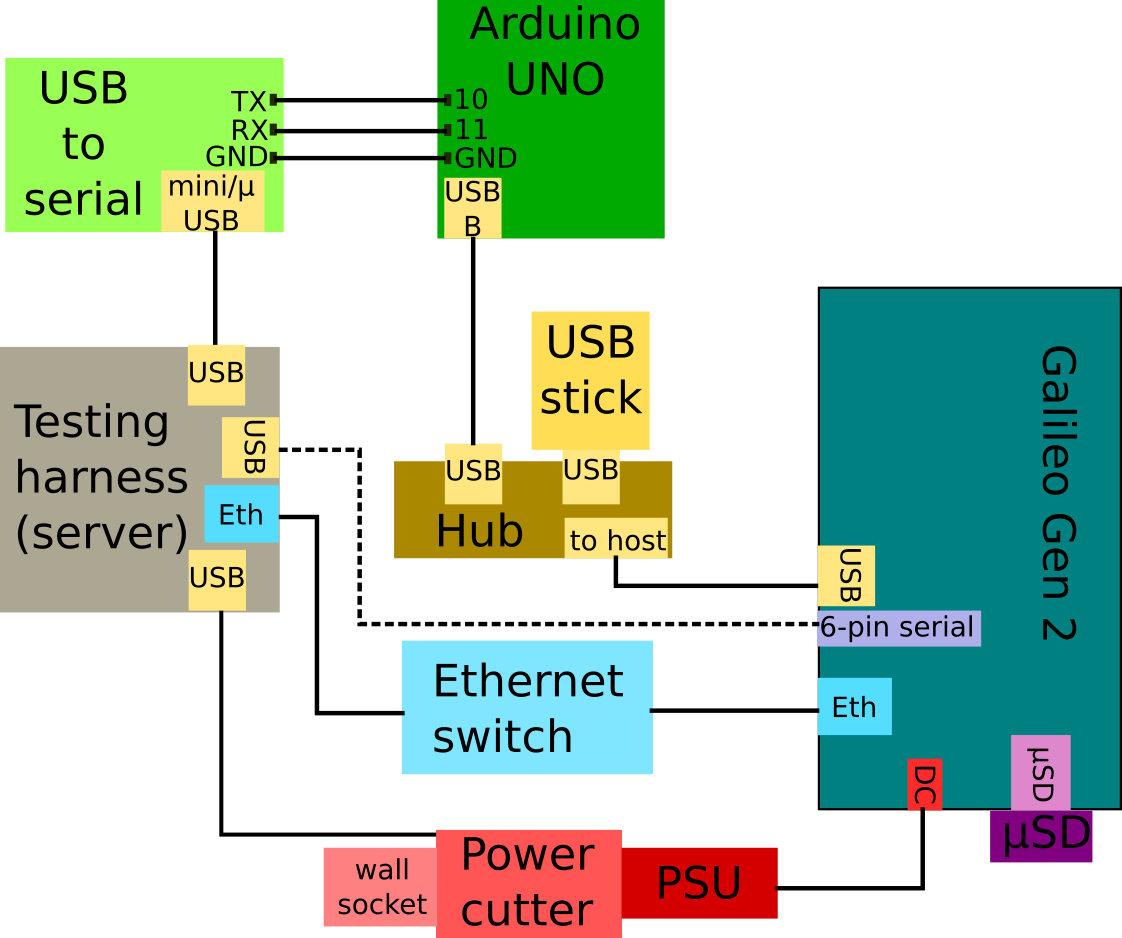
\includegraphics[width=0.7\linewidth]{galileogen2wiring.png}
	\caption{Galileo Gen 2 wiring diagram}
	\label{fig:galileogen2wiring}
\end{figure}

\subsection{Debian on Galileo Gen 2}

The following instructions are based on the preliminary work by Igor Stoppa in creating a bootable SD-card Debian image with persistent storage for the first generation Galileo. Several modifications and additions had to be made to his instructions but the basic idea has remained the same. The main difficulty is finding a Linux distribution which is bootable with an i586 device, as almost all "32-bit" distributions are using at least i686 architecture. Additionally, the kernel configuration required for Galileo Gen 2 had to be searched experimentally, to get all the features required for AFT-integration. The end result is an image which can be booted from both an SD-card or a USB-stick.

The high-level workflow is as follows:
\begin{enumerate}
\label{galileodebianhighlevel}
\item Prepare a 32-bit Debian Virtualbox virtual machine
\item Build a custom Linux kernel using BSP provided by Intel
\item Using debootstrap, prepare the base OS
\item Add other required programs and configuration to the image.
\item Manually construct the boot partition using the custom kernel and EFI GRUB from a Galileo Gen2 image provided by Intel.
\end{enumerate}

The instructions have been tested on 18.11.2015 using a Fedora 22 host machine, 32-bit Debian 8.2 and VirtualBox 5.0.10.

In the following subsections the instructions are described in more detailed manner.

\subsubsection*{Virtualmachine creation}
\begin{enumerate}
\item Using VirtualBox, create a new Debian (32 bit) virtualmachine with 2 GB RAM and 50 GB dynamically allocated VDI harddrive. \note You have to enable a NAT network adapter in the VM settings to have an internet connection inside the VM guest. 

It is recommended to enable also bidirectional shared clipboard and drag'n'drop support.

\item Add a 32-bit Debian installation media in the virtual CD-drive of the VM, start the VM and install it following the installer instructions.

\item Remove the installation media from the virtual CD-drive and restart the VM.

\item Once booted, start a terminal and \cmd{su} to root terminal. \note If you are behind a proxy, it is recommended to set the settings at this point in \cmd{.bashrc}.

\item Comment out CD/DVD-entries in 
\begin{lstlisting}
vi /etc/apt/sources.list
\end{lstlisting}

\item Install required packages to the Debian system: 
\begin{lstlisting}
apt-get install debootstrap vim build-essential binutils git gawk chrpath kernel-package fakeroot libncurses5-dev gparted dkms
\end{lstlisting}

When prompted about the version of kernel config, it is recommended to use the package maintainer's.

\item Install VirtualBox guest additions to the guest and the host systems using instructions from \href{https://www.virtualbox.org/manual/ch04.html}{VirtualBox manual}.

\item Create a shared folder between the host and the VM. In these instructions the folder is named \cmd{shared} on both the host, and the guest machine, under the root home.

\item Download and unpack the SDCard tarball from \url{https://downloadcenter.intel.com/download/24355/Intel-Arduino-IDE-1-6-0} . At the time of writing, the file was named \cmd{SDCard.1.0.4.tar.bz2}

\item copy the extracted \cmd{image-full-galileo}-folder to the shared folder. The folder should contain at least \cmd{grub.efi}, and \cmd{boot/grub/grub.conf}.
\end{enumerate}

\subsubsection*{Kernel construction}
\begin{enumerate}
\item Enter the virtualmachine, start a terminal and switch to root shell using \cmd{su}

\item Download Intel Quark Board Support Package (BSP) sources from  \url{https://downloadcenter.intel.com/download/23197/Intel-Quark-BSP} using eg. \cmd{wget} .

\note At the time of writing the latest version (v. 1.20) had a non-existing base commit ID. Therefore an older version (eg. 1.10) must be used.

\item Unpack the BSP using 
\begin{lstlisting}
7za e *.7z; tar xvf quark_linux_*.tar.gz -C bsp
\end{lstlisting}

\item Git clone the latest stable kernel repository 

\cmd {git clone https://git.kernel.org/pub/scm/linux/kernel/git/stable/linux-stable.git}

\item Checkout the commit SHA found inside \cmd{<bsp>/quark\_linux\_v3.8.7+v1.1.0/upstream.cfg}
\begin{lstlisting}
git checkout 531ec28f9f26f78797124b9efcf2138b8974a1e
\end{lstlisting}

\item Apply the patches required for Galileo Gen2: 
\begin{lstlisting}
git am ../bsp/quark_linux_v3.8.7+v1.1.0/*.patch
\end{lstlisting}

\item Copy the provided kernel config from the stick \cmd{Galileov2/.config} to the kernel repository root.

\item If you wish to customize the kernel configuration, use \cmd{make menuconfig}. For example, adding all the USB-drivers may be desirable.

\item Compile kernel: 
\begin{lstlisting}
fakeroot make-kpkg --initrd  kernel_image modules_image}
\end{lstlisting}  
The .deb package should appear on one folder \textit{above} your working directory.
\end{enumerate}

\subsubsection*{Debian base construction}
\begin{enumerate}
\item Create the empty image file and start partitioning 
\begin{lstlisting}
dd of=galileoimage.img bs=1 count=0 seek=2G; losetup -f galileoimage.img; gparted /dev/loop0
\end{lstlisting}

\item Using gparted, first add a partition table (msdos is fine) and then add 3 partitions: fat32 100MB, linux-swap 500MB, and ext4 the rest. Finally, add \cmd{boot} and \cmd{esp} flags to the fat32 partition.

\item Mount the partitions 
\begin{lstlisting}
mkdir usb_boot; mkdir usb_root; mount /dev/loop0p1 usb_boot; mount /dev/loop0p3 usb_root
\end{lstlisting}

\item Prepare the base system using debootstrap: 
\begin{lstlisting}
debootstrap --arch i386 stable usb_root http://http.debian.net/debian
\end{lstlisting}

\item Rest of the preparation of the chroot environment: 
\begin{lstlisting}
mount --bind /dev usb_root/dev; mount --bind /dev/pts usb_root/dev/pts; cp linux-image*.deb usb_root/root/
\end{lstlisting}
\end{enumerate}

\subsubsection*{Image configuration}
\begin{enumerate}
\item In root shell home, copy the \cmd{authorized\_keys}-file from the usb-stick to the chroot root home: 
\begin{lstlisting}
cp <authorized_keys> usb_root/root/authorized_keys
\end{lstlisting}

\item Start the chroot environment: 
\begin{lstlisting}
chroot usb_root
\end{lstlisting}

\item Install packages required for maintenance: 
\begin{lstlisting}
apt-get install locales ntp openssh-server vim initramfs-tools net-tools bash-completion python python-pip nfs-common nfs-server nano git bmap-tools parted attr gdisk tree
\end{lstlisting}

\item Add the serial terminal: 
\begin{lstlisting}
echo "t0:2345:respawn/sbin/getty -L 115200 ttyS1 vt102" > /etc/inittab
\end{lstlisting}

\note: The terminal interface (\cmd{ttyS1}) depends on the BSP version. This has been tested for 1.10 but an earlier version may use \cmd{ttyQRK1}.

\item Set the password for root user: \cmd{passwd}

\note: The root password in support images so far has been \cmd{rootme}

\item Set the hostname 
\begin{lstlisting}
echo "Debian-Galileov2" > /etc/hostname
\end{lstlisting}

\item Add the hostname to name resolution in \cmd{etc/hosts}:
\begin{lstlisting}
127.0.0.1	localhost Debian-Galileov2
::1		localhost ip6-localhost ip6-loopback Debian-Galileov2
\end{lstlisting}

\item Configure network interface(s) \cmd{vim /etc/network/interfaces}:
\begin{lstlisting}
auto eth0
iface eth0 inet dhcp
\end{lstlisting}
\note It is a good idea to add multiple network interfaces (\cmd{eth1, eth2, ...}) if you want to use the same stick in multiple devices.

\item Permit root login over ssh: 
\begin{lstlisting}
echo "PermitRootLogin yes" >> /etc/ssh/sshd_config
\end{lstlisting}

\item Add ssh-key: 
\begin{lstlisting}
mkdir -p /root/.ssh; chmod 700 /root/.ssh; mv /root/authorized_keys /root/.ssh/; chmod 600 /root/.ssh/authorized_keys
\end{lstlisting}

\item Create NFS and testable image mount point directories: 
\begin{lstlisting}
mkdir /mnt/img_data_nfs; mkdir /mnt/super_target_root; mkdir /mnt/target_root
\end{lstlisting}

\item Add entries to \cmd{/etc/fstab}: \cmd{vim /etc/fstab}:
\begin{lstlisting}
/dev/sda3 / ext4 defaults 0 0
192.168.30.1:/home/tester /mnt/img_data_nfs nfs rsize=8192,wsize=8192,timeo=14,intr,nolock,auto
\end{lstlisting}

\item Install the kernel package: 
\begin{lstlisting}
dpkg -i /root/*.deb
\end{lstlisting}

\item Fix \url{https://bugs.debian.org/cgi-bin/bugreport.cgi?bug=738575}. The command replaces every \cmd{lock} instruction with a \cmd{nop}. This works because Quark is a single-core processor: 
\begin{lstlisting}
for i in `/usr/bin/find /lib -type f -name *pthread*so`; do cp \$\{i\} \$\{i\}.bak; sed -i "s/\bl xf0\bl x0f\bl xb1\bl x8b/\bl x90\bl x0f\bl xb1\bl x8b/g" \$\{i\}; done
\end{lstlisting}

\item Leave the chroot environment using \cmd{ctrl+d}

\item Copy the EFI files from shared folder: 
\begin{lstlisting}
mkdir -p usb_boot/EFI/BOOT; \linebreak cp shared/image-full-galileo/grub.efi usb_boot/EFI/BOOT/bootia32.efi; \linebreak cp -a shared/image-full-galileo/boot usb_boot
\end{lstlisting}

\item Copy the kernel files to boot partition: 
\begin{lstlisting}
cp usb_root/boot/* usb_boot
\end{lstlisting}

\item Modify the \cmd{usb\_boot/boot/grub/grub.conf}, make the following entry and remove the others:
\begin{lstlisting}
title Debian
    root (hd0,0)
    kernel /vmlinuz-3.8.7+ root=/dev/sda3 3 console=ttyS1,115200n8 earlycon=uart8250,mmio32,$EARLY_CON_ADDR_REPLACE,115200n8 vmalloc=3844M reboot=efi,warm apic=debug rw LABEL=boot debugshell=5
    initrd /initrd.img-3.8.7+
\end{lstlisting}
\note You may have to modify the \cmd{vmlinuz-3.8.7+} and \cmd{initrd.img-3.8.7} to correspond your kernel and initrd files.

\note If you want to boot the image from a SD-card, modify the \cmd{root=/dev/sda3} option to point to the SD-card: \cmd{root=/dev/mmcblk0p3}.

\item Unmount everything and copy the image to the shared folder. 
\begin{lstlisting}
umount /dev/loop0p1; umount /dev/loop0p3; cp galileoimage.img shared
\end{lstlisting}

\item Poweroff the VM.

\item Inside the host system, dd the \cmd{galileoimage.img} to a USB-stick: 
\begin{lstlisting}
sudo dd if=shared/galileoimage.img of=/dev/sdX bs=8M
\end{lstlisting}

\note modify the X to correspond your USB-stick device which can be found using eg. \cmd{lsblk}.
\end{enumerate}

\section{Intel Edison}
\label{edison}

Intel Edison is a development platform intended for wearable devices. It is a SoC with two Intel Atom cores and one Intel Quark core, GB of internal RAM and integrated Bluetooth and Wi-Fi. The Atoms are normal x64 cores while the Quark is roughly an i586 processor.

Edison can be mounted on an Arduino development kit which provides Arduino UNO compatible pin layout. The development board also has a USB-serial interface, a mechanical switch to select between a micro-USB device controller  and a normal USB socket, a DC plug and a microSD socket.

Edison uses a hacked U-Boot for hardware initialization. 

From flashing perspective, Edison is closer to a mobile phone or similar "gadget" device than a complete PC. The OS image is written using DFU.

\subsection{USB-interfaces}

When an Edison is plugged to a computer, it is first detected as an Intel Merrifield device (\cmd{8086:e005}), which is used to recover the DFU-utility in the firmware. After a few seconds the device disconnects and reconnects as DFU-device, Intel USB download gadget (\cmd{8087:0a99}).  At this stage the OS can be flashed. If DFU-communication is not initialized in a couple of seconds, the device disconnects again and finally boots normally. 

After the boot process, the device is detected with multiple interfaces with ID \cmd{8087:0a9e}. It can be used as a USB-storage, USB-serial device (at \cmd{/dev/ttyACM\textit{X}}) and as a USB-network interface.

The USB-network interface is used for network connectivity. This interface has to be configured on both the image under test and the testing harness. Network configuration is handled by AFT \ref{aft}.

The USB-network interface of the Edison gets a random MAC-address every time the image is flashed. This also causes the network interface on the testing harness being recreated and renamed.

If there are multiple Edisons attached to the testing harness, the only way to differentiate between them is the USB-tree or USB-paths. Using the paths, each physical USB-port can be differentiated from each other.

\subsection{CI-integration}

Integrating Edisons to the testing automation requires a way to power off and on the device programmatically.

The best solution would be to find USB-hubs that supports Linux kernel's USB power options at \cmd{/sys/bus/usb/devices/usb1/power/} on per-port accuracy. Unfortunately this kind of USB-hubs are extremely difficult to find.

An implemented alternative is to use a power cutter on USB-cable's +5V line. Because the device is powered by USB, the power cutter also shuts down the device. This requires exposing the +5V cable, stripping it, and attaching the newly open ends to a USB-controlled relay, as instructed in figure \ref{fig:usbpower}.

The USB-serial interface can be used for boot console recording at 115200 bauds.
\begin{figure}
	\centering
	\begin{minipage}[c][0.5\textheight][t]{0.49\textwidth}
	\centering
	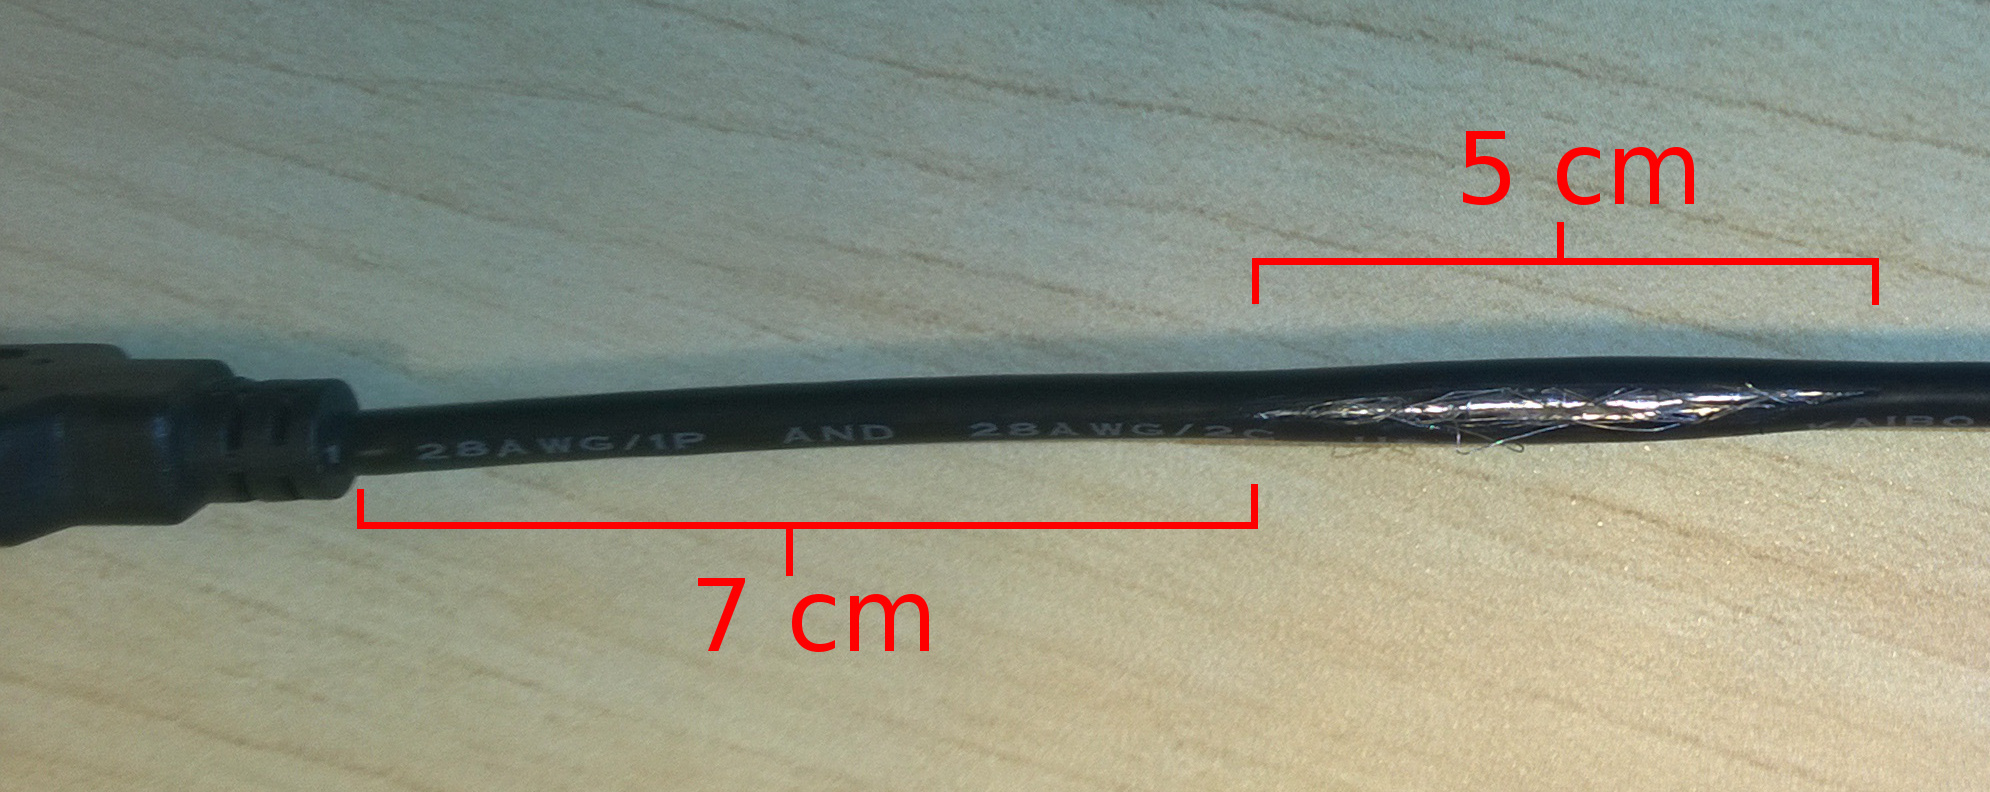
\includegraphics[width=\linewidth]{edisonwire1.jpg}
	
	1. Expose the wire shielding by cutting a 5 cm slice through the jacket, about 7 cm from the USB-A plug.
	\end{minipage}
	\begin{minipage}[c][0.5\textheight][t]{0.49\textwidth}
	\centering
	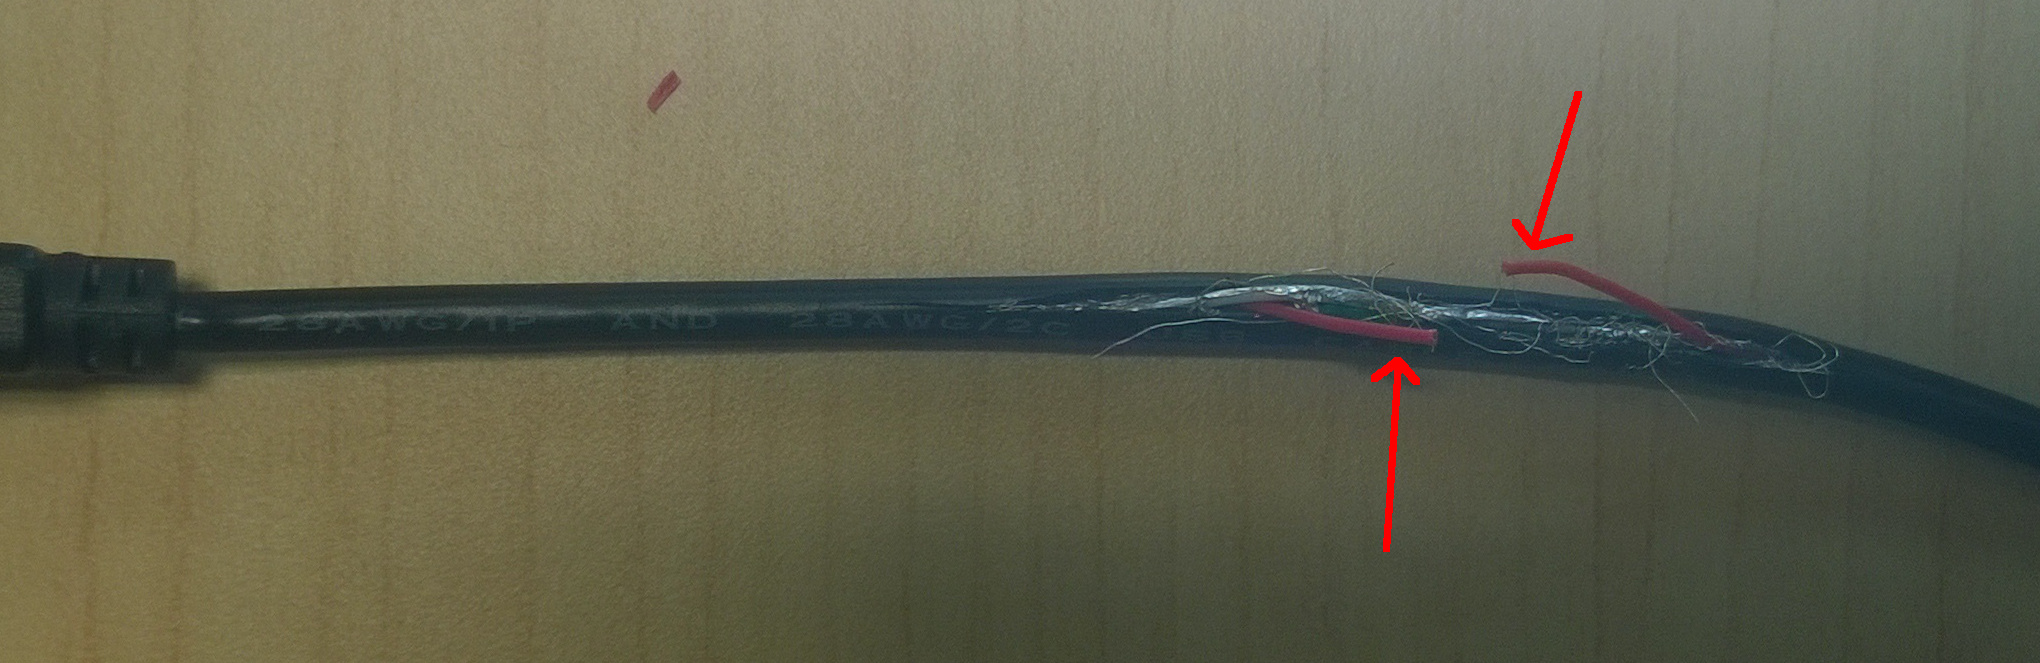
\includegraphics[width=\linewidth]{edisonwire2.jpg}
	
	2. Strip the shielding carefully.	
	Expose the red wire (+5V) and cut it in half.
	\end{minipage}
	\begin{minipage}[c][0.5\textheight][t]{0.49\textwidth}
	\centering
	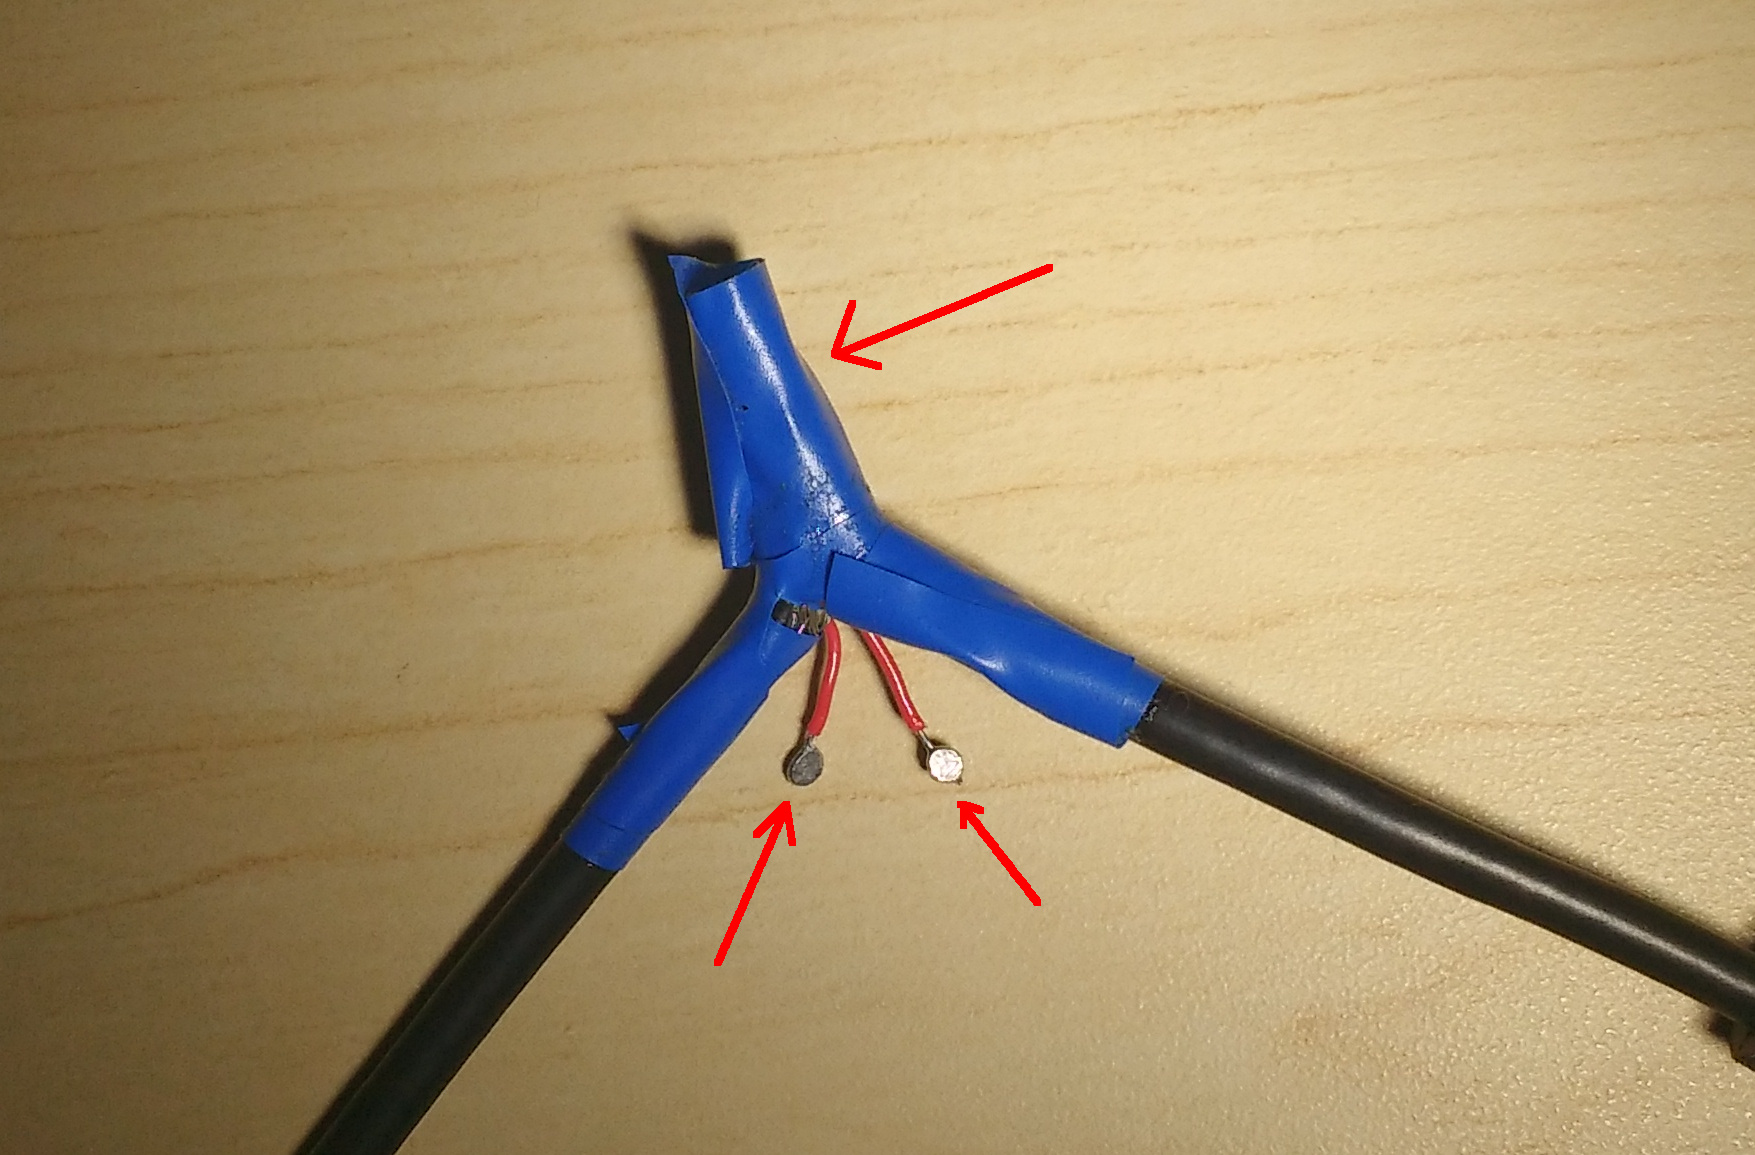
\includegraphics[width=\linewidth]{edisonwire3.jpg}
	
	3. Strip the wire, solder small beads of tin on the tips and    flatten the beads with pliers or similar tool.
	Cover the cut with electrical tape.
	\end{minipage}
	\begin{minipage}[c][0.5\textheight][t]{0.49\textwidth}
	\centering
	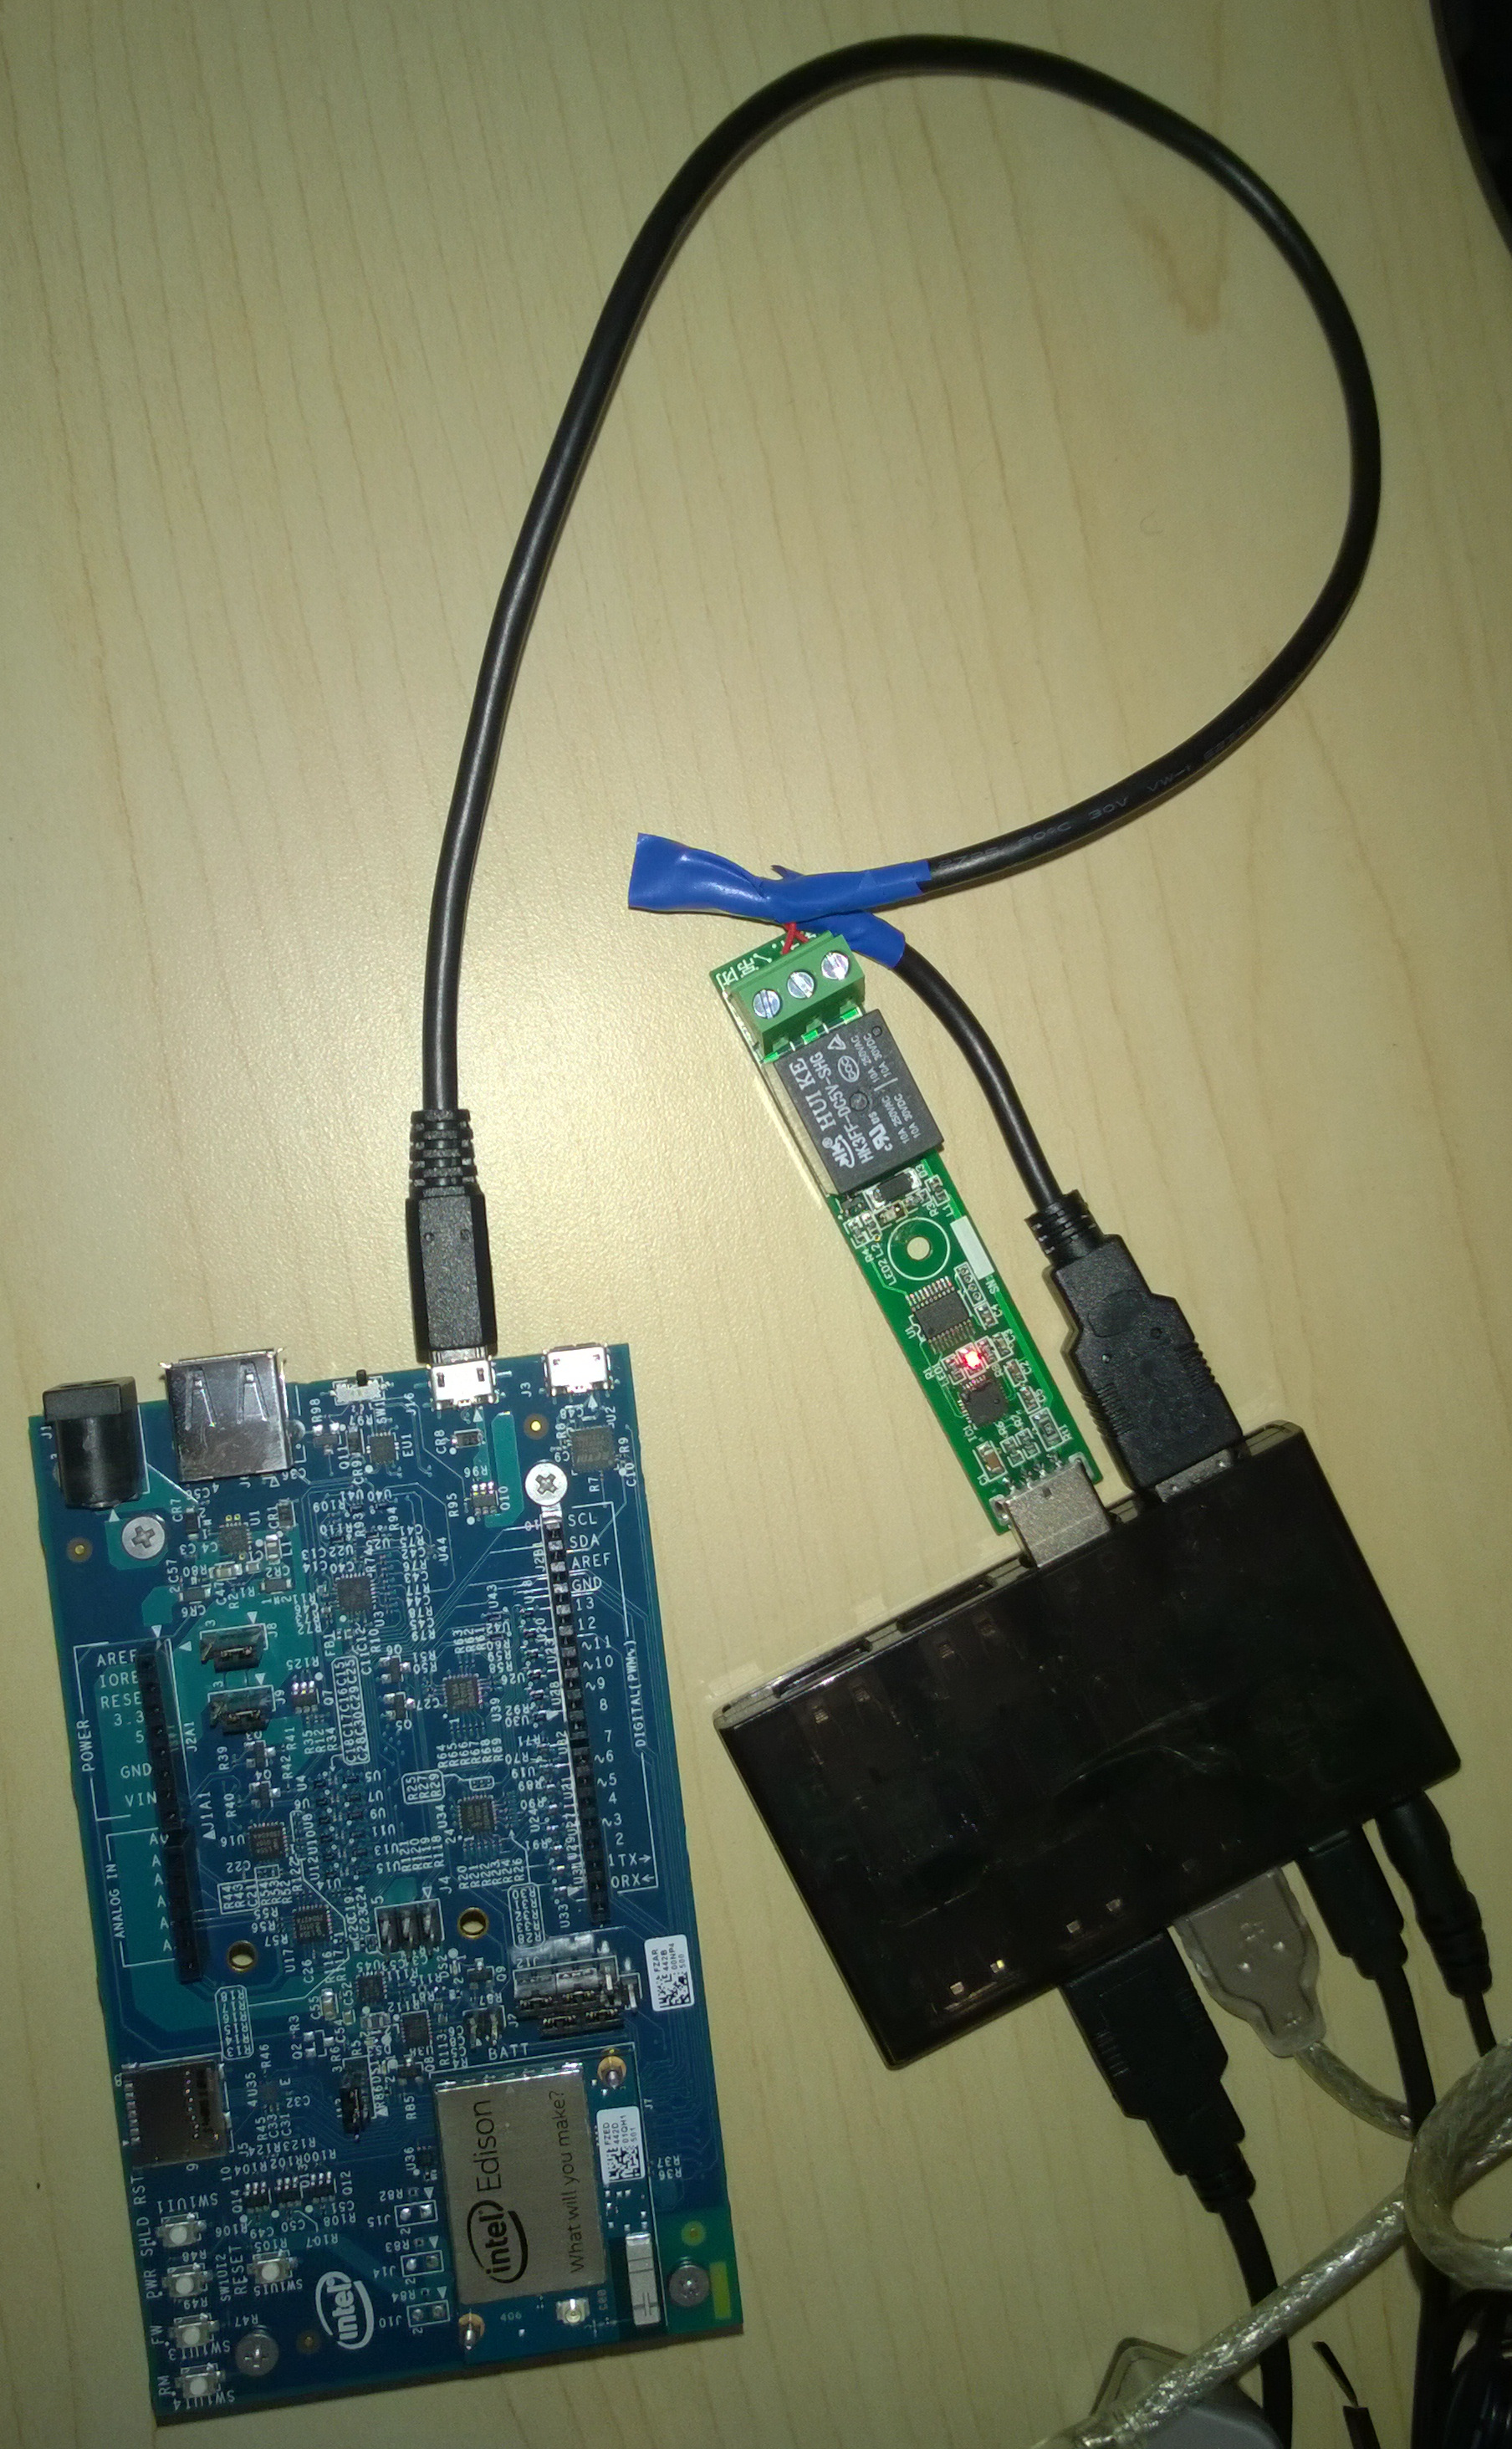
\includegraphics[height=0.35\textheight]{edisonwire4.jpg}
	
	4. Final setup.
	\end{minipage}
	\caption{USB-power cutter cable.}
	\label{fig:usbpower}
\end{figure}

\newpage
\section{Beaglebone Black}
Beaglebone Black is an open-source hardware development board with a 32-bit 1GHz Cortex-A8 ARM CPU and 512 MB ram. The board also has two 200MHz 32-bit microcontrollers, which can be used to offload tasks from the main CPU. Depending on revision, it has either 2 gigabytes (rev B) or 4 gigabytes (rev C) of internal storage. It has microSD slot, A-type and mini USB ports, microHDMI connector for video and audio, 100 megabit ethernet and a 6-pin serial output. It can be powered through either mini-usb port or 5.5mm 5V jack.

Beaglebone is a gadget-like device that uses U-boot for initialization. It however requires a support image for flashing due to the official flashing procedure requiring manual steps.

\subsection{CI-integration}

\begin{figure}[h]
	\centering
	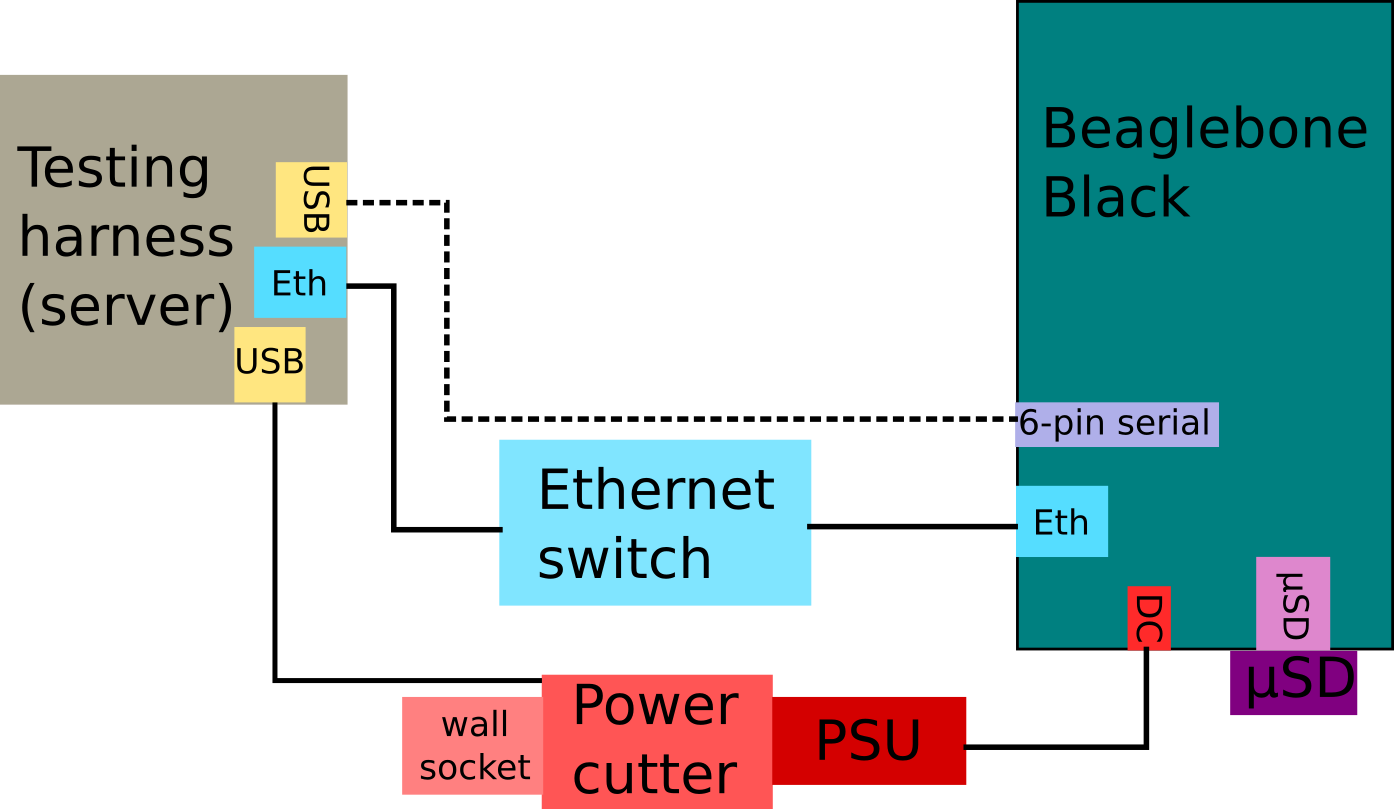
\includegraphics[width=0.7\linewidth]{beaglebonewiring.png}
	\caption{Beaglebone Black wiring diagram}
	\label{fig:minnowwiring}
\end{figure}

Beaglebone Black is effectively a hybrid PC-like/gadget device for the purposes of this documentation. It lacks bios, and its default flashing protocol is closer to a gadget flashing protocol like what Edison uses, rather than what the PC-like devices use. However, as the default flashing protocol requires manual steps (user has to press a button during boot, after which the device copies image present on SD card into internal storage), it requires a support image for automatic flashing.

The support image is stored on the testing harness, and accessed over nfs. This reduces failure points, as USB sticks have been known to fail due to frequent power cuts. This also makes support image updates easier, as the root filesystem can be updated over SSH on the testing harness. Fundamentally however there is nothing preventing the use of USB based support image, so AFT can be modified to support this if necessary.

The internal ethernet adapter is used for network connectivity. Both the support image and tests are accessed through network.

Unlike other devices with serial outputs, a serial cable must be connected to the device's 6-pin serial output. The commands to boot over nfs are sent through serial cable, so it must be present for flashing to work. Device output is additionally recorded over serial output for easier debugging. Recommended rate is 115200 bauds.

The microSD-card is used for the target image. While internal storage could be used, this allows easier device rescue in case of a image with a bad bootloader. Reflashing SD-card with a valid bootloader is easier than flashing the internal storage with a valid bootloader. There is also the minor benefit that replacing faulty SD-card is easier than modifying AFT to support SD-card after eMMC failure.

A power cutter such as Cleware cutter is used to cut the device power when needed.

\subsection{Preparing Beaglebone Black}

By default, BeagleBone Black boots from the internal eMMC storage. Booting from SD card requires user to press a button on the board during the boot. If the eMMC bootloader is removed however, BeagleBone will check the SD card for a bootloader. This allows the device to boot from the SD card, where the testable image will be stored.

As the Beaglebone doesn't seem to expose its boot partition to host computer when connected, we need to connect to the device with either serial cable or over ssh, and overwrite the boot files.

\begin{enumerate}

\item Connect the Beaglebone Black to a computer with a micro-USB cable. 

\item Once BeagleBone Black has booted, a new network interface should show up under \cmd{ifconfig}.

\item SSH into the device, using the network interface ip address plus one (e.g. if the interface ip is 192.168.7.1, device ip is 192.168.7.2) and user 'debian'. Password should be 'temppwd'.

\note The default user/password might have changed after writing this. If this is the case, either find out the user and password, or connect to the device using serial cable and reboot the device. It should show the default user/password above login prompt. At this point, you can continue using the serial connection rather than SSH connection.

\item Destroy the partition by executing 

\begin{lstlisting}
dd if=/dev/zero of=/dev/mmcblk0 bs=4M count=10
sync
\end{lstlisting}

This writes 40 megabytes worth of zeros into the eMMC, which should be more than enough to destroy the boot partition.

\note If you have SD card connected, the eMMC should be \cmd{/dev/mmcblk1} instead of \cmd{/dev/mmcblk0}. It's best not to connect SD card at this point to avoid confusion

\item Copy bootloader files, \cmd{MLO} and \cmd{u-boot.img}, into the SD card boot partition, or flash the SD card with an functioning image. The test automation USB stick should have the necessary bootloader files, but any valid bootloader should do. See \ref{part_sd} on how to partition the SD card correctly.

\end{enumerate}

\note In case a bad image ends up being flashed into the SD card, Beaglebone Black will fail to boot as no working bootloader is present. To fix this, flash the SD card with a working image.

\subsection{Partitioning SD-card}
\label{part_sd}
AFT assumes that the SD-card is partitioned properly. When adding a new device, or replacing old SD-card, the SD-card must have at least two partitions: 64 megabyte boot partition and at least 4 gigabyte root partition.

These following steps use \cmd{fdisk}, but any partitioning software will do.

\begin{enumerate}

\item Verify that the card is unmounted

\item Run fdisk on the SD-card

\begin{lstlisting}
sudo fdisk /dev/sdX
\end{lstlisting} 

where \cmd{/dev/sdX} is the device file for your SD-card. This can be found by using e.g. \cmd{lsblk}.

\item Use the following commands to partition the card:

\begin{lstlisting}
o  -- creates new dos partition table
n  -- add new partition
enter  -- use default (primary partition)
enter  -- use default (first partition)
enter  -- use default (default starting position)
+64M -- set partition size as 64 megabytes
a -- set first partition as bootable
n -- add new partition
enter -- use default (primary partition)
enter -- use default (second partition)
enter -- use default (default starting position
enter -- use default (any remaining space is added to the partition)
t -- change partition type
1 -- first partition 
6 -- Fat16 partition
t -- change partition t
2 -- second partition 
83 -- Linux partition
p -- print the partition table (optional)
w -- write the results
\end{lstlisting}

If the commands were entered correctly, the partition table (press \cmd{p} to print the partition table) should look something like this:

\begin{tabular}{c c c c c c c c}
Device & Boot & Start & End & Sectors & Size & Id & Type \\
/dev/sdb1  & * & 2048 & 133119 & 131072 & 64M & 6 & FAT16 \\
/dev/sdb2  &   & 133120 & 15130623 & 14997504 & 7,2G & 83 & Linux \\
\end{tabular}

If the partition table looks correct, you can write the results by entering \cmd{w}. You may need to run \cmd{partprobe} so that the kernel sees the new partitions.

\item After the disk has been partitioned, file systems must be created on the card. While AFT recreates file systems on flashing, the SD card must have a valid bootloader present on the boot partition or the initial boot fails. 

\begin{lstlisting}
sudo mkfs.fat /dev/sdX1
sudo mkfs.ext4 /dev/sdX2 (optional - AFT will recreate the file system on flashing)
\end{lstlisting}

Where \cmd{/dev/sdX} once again is the SD-card device file
\end{enumerate}

\subsection{Debian for Beaglebone Black}
\label{bbbdebian}

Unlike other devices, Beaglebone Black uses its support image over nfs. This is due to an effort to minimize single point of failures, as USB-sticks have been known to fail due to frequent power cuts. 

The following steps can be run on either personal computer or the testing harness, as long as the resulting root filesystem directory is copied to testing harness with appropriate ownership. The steps however assume that the commands are run on the testing harness as root. Adjust paths and add sudos where necessary.


\begin{enumerate}
\item Download Debian 8.2 "Jessie" image from \url{http://www.beagleboard.org}.

\note Newer images should work as well, but some of the following steps might be inaccurate.

\item Extract the root filesystem from the image file


\item Extract the root filesystem from the image

\begin{lstlisting}
mkdir temp
losetup --show -f -P bone-debian-8.2-tester-2gb-armhf-2015-11-12-2gb.img
mount /dev/loop0p2 temp
cp -R temp/* /home/tester/support_fs/beaglebone/ 
umount temp
losetup -D 
rmdir temp
\end{lstlisting}

Replace \cmd{/dev/loop0} with the loop device that was printed when initially creating the loop device, and \cmd{p2} with the actual root filesystem partition.

\note \cmd{losetup -D} Detaches all loop devices

\item Remove the connman service

Connman service resets the ip during boot process, which causes the boot to fail as connection to nfs server is lost.


\begin{lstlisting}
rm /home/tester/support_fs/beaglebone/etc/systemd/system/multi-user.target.wants/connman.service
\end{lstlisting}

\note It may also be necessary to remove connman symlinks from \cmd{etc/rd?.d} folders, where ? is a number.


\item Add ssh key to the image

\begin{lstlisting}
mkdir /home/tester/support_fs/beaglebone/root/.ssh
cp id_rsa_testing_harness.pub /home/tester/support_fs/beaglebone/root/.ssh/authorized_keys
chmod 700 /home/tester/support_fs/beaglebone/root/.ssh
chmod 600 /home/tester/support_fs/beaglebone/root/.ssh/authorized_keys
\end{lstlisting}


\item Change ownership to nobody

As the nfs uses root squash, root access is mapped to user 'nobody'.

\begin{lstlisting}
chown -R nobody:nobody /home/tester/support_fs/beaglebone
\end{lstlisting}



\item Add the following to testing harness \cmd{/etc/exports}

\begin{lstlisting}
/home/tester/support_fs 192.168.30.0/24(crossmnt,rw,sync,root_squash,no_subtree_check) 
\end{lstlisting}

\note \cmd{/etc/exports} is whitespace sensitive. Only add space between the direcory path and ip address.

\item Make sure that the settings are updated by running the following command.

\begin{lstlisting}
exportfs -vr
\end{lstlisting}

\item Boot\ref{bbbboot} the support image once

\item Remove the new export from \cmd{/etc/exports} and run the update command

The change in \cmd{/etc/exports} changes the nfs from read-only to read/write. This allows the support os to write any configuration files and do whatever changes it needs during the first boot. Without this step, at least the ssh service will fail to start. After one succesful run, the export can be removed so that the file system is read-only. This is recommended for security reasons.


\end{enumerate}

\subsubsection{Alternate way of mounting the image}

If the \cmd{losetup}-command does not work for some reason, the following command can be used instead.

\begin{lstlisting}
mount -o loop,offset=<offset value here> bone-debian-8.2-tester-2gb-armhf-2015-11-12-2gb.img temp/
<copy the root filesystem as above>
umount temp
\end{lstlisting}

The offset can be calculated by printing the partition table with fdisk and then multiplying the starting position by sector size

\begin{lstlisting}

fdisk -l bone-debian-8.2-tester-2gb-armhf-2015-11-12-2gb.img 
Read sector size and root system start position
Multiply these values with each other

\end{lstlisting}

Example output (image names have been edited as they were too long):

\cmd{Disk name-too-long.img: 1,7 GiB,  1782579200 bytes, 3481600 sectors} \\
\cmd{Units: sectors of 1 * 512 = 512 bytes} \\
\cmd{Sector size (logical/physical): 512 bytes / 512 bytes} \\
\cmd{I/O size (minimum/optimal): 512 bytes / 512 bytes} \\
\cmd{Disklabel type: dos} \\
\cmd{Disk identifier: 0x00000000} \\


\cmd{\begin{tabular}{c c c c c c c c}
Device & Boot & Start & End & Sectors & Size & Id & Type \\
name-too-long.img1 & * & 2048 & 198655  & 196608 & 96M & e & W95 FAT \\
name-too-long.img2 &   & 198656 & 3481599 & 3282944 &  1,6G & 83 & Linux \\
\end{tabular}
}

Here the sector size is 512 bytes, and the root filesystem starts at sector 198656. Now we can calculate the offset: 512*198656 = 101711872 




\subsection{Booting into the service mode}
\label{bbbboot}

\begin{enumerate}
\item Open screen

\begin{lstlisting}
screen /dev/ttyUSBX 115200, -ixon,-ixoff
\end{lstlisting}
where \cmd{/dev/ttyUSBX} is the device file for the serial port.

\item Power on the device

\item Immediately after powering on the device, press space\footnote{The button has changed at least once after writing this document, so this might have changed by the time you read this} to interrupt the regular boot to enter u-boot console

\item Enter the following commands to boot the device over nfs

\begin{lstlisting}
setenv autoload no
dhcp
setenv bootargs console=ttyO0,115200n8 root=/dev/nfs nfsroot=${serverip}:/home/tester/support_fs/beaglebone,vers=3 rw ip=${ipaddr}
tftp 0x81000000 support_fs/beaglebone/boot/vmlinuz-4.1.12-ti-r29
tftp 0x80000000 support_fs/beaglebone/boot/dtbs/4.1.12-ti-r29/am335x-boneblack.dtb
bootz 0x81000000 - 0x80000000
\end{lstlisting}

\note You may need to modify the paths above if you use different installation location or support image

\note 0x81000000 and 0x80000000 are the memory locations where the kernel and device tree binaries are downloaded. It is important that these do not overlap (e.g. 0x80000000 + device tree binary size must be smaller than 0x81000000). The memory addresses themselves are somewhat arbitrary, but they have been tested to work.

\end{enumerate}

\section{VirtualBox}

VirtualBox is open-source hypervisor for x86 computers. It is currently developed primarily by Oracle Corporation. It is available on Windows, Linux, OS X and Solaris, with ports available to FreeBSD and Genode.

VirtualBox can be used to run 32- and 64-bit x86 based Ostro images. Currently only 64-bit corei7-64 images are used for CI testing.

\subsection{CI-integration}

As the testable image is run in a virtual machine, there are no additional physical requirements for the testing setup. The VirtualBox setup however requires several configuration changes. Note that the following commands assume root privileges for terseness; you may need to use sudo or equivalent command.

\begin{enumerate}

\item
First of all, VirtualBox must be installed

\begin{lstlisting}
zypper install virtualbox
\end{lstlisting}

\item 
After installation VirtualBox kernel modules may not be active. You can list the active modules by running

\begin{lstlisting}
lsmod | grep vbox
\end{lstlisting}

The following modules should be present: \cmd{vboxdrv}, \cmd{vboxnetapd}, \cmd{vboxnetflt} and \cmd{vboxpci}. If one or more of them are missing, you can use the following commands to load the missing modules

\begin{lstlisting}
modprobe vboxdrv
modprobe vboxnetctl
modprobe vboxnetflt
modprobe vboxpci
\end{lstlisting}

\note \cmd{vboxnetctl} has different name than the kernel modules. This is intentional

\item
Linux Kernel-based virtual machine (KVM) interferes with VirtualBox and needs to be shut down. You can check if the KVM is currently loaded by running

\begin{lstlisting}
lsmod | grep kvm
\end{lstlisting}

If \cmd{kvm-intel} or \cmd{kvm-amd} is present (depending on your system CPU), you can use one of the following commands to disable the module

\begin{lstlisting}
sudo modprobe -r kvm-intel
sudo modprobe -r kvm-amd 
\end{lstlisting}

\item 
By default, VirtualBox requires root privileges to run. See \ref{virtualboxnoroot} for more information how to configure the system to avoid this requirement.

\item
AFT sets the testable .ova appliance into bridged mode for testing. This means we need to create a virtual network interface and modify it to use the \cmd{dnsmasq} for ip address allocation.

\begin{lstlisting}
VBoxManage hostonlyif create
\end{lstlisting}

The virtual network interface by default uses a VirtualBox based DHCP server for IP-address allocation. As the testing setup already uses \cmd{dnsmasq} for this, we need to remove the default DHCP server and modify \cmd{dnsmasq} to also allocate IP addresses for the VirtualBox.

Removing the DHCP server can be done with the following commands

\begin{lstlisting}
VBoxManage list dhcpservers
VBoxManage dhcpserver remove --netname <network name>
\end{lstlisting}

\cmd{dnsmasq} must be configured to allocate IPs for the virtual adapter as well. You first need to get the interface name by running

\begin{lstlisting}
VBoxManage list hostonlyifs
\end{lstlisting}

The name seems to be \cmd{vboxnet0} and the ip address 192.168.56.1 by default, assuming they weren't already taken. It is best to verify this however. The interface name and the ip address range must be then added into \cmd{/etc/dnsmasq.conf}. 

\begin{lstlisting}
interface=vboxnet0
dhcp-range=192.168.56.2,192.168.56.254,10m
\end{lstlisting}

Where \cmd{vboxnet0} is the default name and \cmd{dhcp-range} has the default ip address. Replace these if necessary.

\item
AFT uses \cmd{guestmount} to mount the VirtualBox hard drive to inject the ssh key. The key needs a correct \cmd{security.ima} extended attribute, or Ostro Integrity Management Architecture (IMA) feature rejects the file. The attribute is set using \cmd{setfattr} command line tool.The tool requires root privileges for this operation. See \ref{virtualboxsetfattr} for more information how to use the tool if the tester account does not have root privileges.

Guestmounted files by default are visible only to the user who mounted the file; any other user will get a 'permission denied' error, including root, when attempting to access these files. As AFT must work without root privileges (when the system has been properly configured), it always uses \cmd{-o allow\_other} -option when mounting the VirtualBox hard drive to allow other users to see the mounted files. This is required so that the \cmd{setfattr} can modify the file attributes, as this command is always executed as root. This option however is unavailable without modifying FUSE (filesystem in userspace) configuration file. This means the following line must be added (if not already present) into \cmd{/etc/fuse.conf} (\note The configuration file may not be present in the system. You need to create it if this is the case)

\begin{lstlisting}
user_allow_other
\end{lstlisting}



\end{enumerate}





\newpage
\appendix
\section{AFT implementation details}
\label{app:aft}

In this appendix, configuration options are detailed. Also, a high level description of most important AFT implementation decisions are explained. 

\subsection{Configuration}

All AFT configuration is done with configuration files stored in \cmd{/etc/aft}.

Configuration files for the testable devices are stored in the subfolder \cmd{devices}. The configuration of a single physical device is combined out of these files.

In the \cmd{test\_plan} folder is the configuration for each AFT test-plan.

\subsubsection*{devices/platform.cfg}
The \cmd{platform.cfg} is the highest level configuration file. It is intended to store settings which are shared between all high-level device-types, ie. PC-devices or gadget-devices.

This is also the place where settings for automatic construction of the device topology can be stored. For example the \cmd{leases\_file\_name} refers to the location of the leases file used by \cmd{dnsmasq}. This file can be used to detect devices attached to the local network in which the PC-devices are kept in.

\subsubsection*{devices/catalog.cfg}
The \cmd{catalog.cfg} is the configuration file describing each device type. These are the options shared by all devices of the same type.

Specifying an option here that is also specified in \cmd{platform.cfg} overrides the option. In general, this is discouraged, as if there is need to override settings, it usually means the setting does not belong in \cmd{platform.cfg}. It can be useful for debugging though.

Each section in \cmd{catalog.cfg} must include at least the \cmd{platform}, \cmd{cutter\_type} and \cmd{test\_plan} options.

The \cmd{platform} option is used to load the correct high-level device configuration from the \cmd{platform.cfg} file. 

The \cmd{cutter\_type} is used to determine the type of cutter used for the devices. At the time of writing the options are \cmd{clewarecutter} and \cmd{usbrelay}.

The \cmd{test\_plan} option is the name of the test plan configuration file under \cmd{test\_plan} folder.

For \emph{PC-devices}, the additional options are as follows:
\begin{itemize}
\item \cmd{target\_device}: The block device the image is flashed to.

\item \cmd{root\_partition}: The partition to which the root of the image ends up after flashing the image. \note this option is only used if there is no disk layout configuration file in the AFT invocation folder.

\item \cmd{disk\_layout\_file}: The partition layout file name. Expected to be found in the working directory of AFT invocation.

\item \cmd{service\_mode}: A pattern which can be used to verify that the device is in service mode, that is, ready to be flashed. Compared against \cmd{/proc/version}.

\item \cmd{test\_mode}: Same as above but for the testing mode, that is, what is seen after the testable image has booted.

\item \cmd{service\_mode\_keystrokes}: The keyboard sequence which switches the BIOS options to service mode.

\item \cmd{test\_mode\_keystrokes}: Same as above but for testing mode.
\end{itemize}

For \emph{Beaglebone Black}, the additional options are as follows:
\begin{itemize}
\item \cmd{service\_mode}: Identical to PC-device option.

\item \cmd{test\_mode}: Identical to PC-device option.

\item \cmd{boot\_partition}: The block device and partition for the boot files. Example: \cmd{/dev/mmcblk0p1}

\item \cmd{root\_partition}: The block device and partition for the root fs. Example: \cmd{/dev/mmcblk0p2}

\item \cmd{support\_fs}: Specifies the path from nfs root to the support fs folder. If nfs root is \cmd{/home/tester/}, then this could be for example \cmd{support\_fs/beaglebone}, assuming the full path on the host system is \cmd{/home/tester/support\_fs/beaglebone}. Note that the lack of initial / is intentional.

\item \cmd{support\_kernel\_path}: Path to kernel image on the support fs, starting from the support fs root. Example path: \cmd{boot/vmlinuz-4.1.12-ti-r29}. Note that the lack of initial / is intentional.

\item \cmd{support\_dtb\_path}: Path to the device tree binary on the support fs, starting from the support fs root. Example path: \cmd{boot/dtbs/4.1.12-ti-r29/am335x-boneblack.dtb}. Note that the lack of initial / is intentional.

\item \cmd{mlo\_file}: The name of the MLO file (second stage bootloader) that will be flashed to the boot partition.

\item \cmd{u-boot\_file}: The name of the u-boot image file (third stage bootloader) that will be flashed to the boot partition.

\item \cmd{root\_tarball}: The name of the tarball that contains the root filesystem that will be flashed  to the root partition.

\item \cmd{dtb\_file}: The name of the device tree binary file that will be flashed to the root partition.

\item \cmd{serial\_bauds}: See description below. This is a mandatory field for Beaglebones, as serial connection is used to pass some commands during initial service mode boot.

\end{itemize}

For \emph{Edison} devices there are no extra device specific options.

For \emph{serial recording}, the add option:
\begin{itemize}
	\item \cmd{serial\_bauds}: The baudrate of the serial connection.
\end{itemize}

\subsubsection*{devices/topology.cfg}

The \cmd{topology.cfg} file contains individual physical device specific information. The options you have to specify here depend on the device type and the power cutter used with it.

Specifying an option here that is also specified in \cmd{platform.cfg} or \cmd{catalog.cfg} overrides the option. In general, this is discouraged, as if there is need to override settings, it usually means the setting does not belong in these configuration files (it is device specific). It can be useful for debugging though.

The mandatory options for all devices are the \cmd{model} and \cmd{id}. The information required to construct a cutter instance specific to the device is also almost certainly required.

The \cmd{model} is the device model. This is used to determine which device type from \cmd{catalog.cfg} is associated with the physical device.

The \cmd{id} is a unique identifier which is used as the name of the lock file associated with the device, when the device is in use. For PC-devices and Beaglebone Blacks this should be the MAC-address. For Edisons this can be anything that is unique.

The options related to \emph{Clewarecutters} are as follows:
\begin{itemize}
\item \cmd{cutter}: The ID of the cutter. This is taped on each cutter but can be also found using the \cmd{clewarecontrol} tool
\item \cmd{channel}: The power socket of the cutter specified with \cmd{cutter}.
\end{itemize}

For \emph{usbrelays} the only required option is \cmd{cutter}. This specifies the ttyUSB device associated with the cutter.

For \emph{PC-devices} the mandatory options are as follows:
\begin{itemize}
\item \cmd{pem\_interface}: the interface used with PEM. The only option at the time of writing is serialconnection.
\item \cmd{pem\_port}: The ttyUSB device for the USB-to-serial adapter connected to the PEM-Arduino.
\end{itemize}

For \emph{Beaglebone Blacks}, \cmd{serial\_port} is mandatory (see below for more details) as the commands required for booting service mode are passed through serial connection

For \emph{Edisons} the mandatory options are as follows:
\begin{itemize}
\item \cmd{edison\_usb\_port}: The USB-bus and -port to which the USB-cable to Edison is attached. This can be found for example from \cmd{dmesg} output when the device powers on:

\begin{lstlisting}
[239158.679601] usb 2-1.1.4.1.4: Product: Edison
\end{lstlisting}

The required value in this case is 2-1.1.4.1.4

\note Do not confuse the usb relay with the actual data cable; we are interested in the data cable values.

\item \cmd{network\_subnet}: A *.*.*.*/30 subnet dedicated for this specific Edison device.
\end{itemize}

For \emph{serial recording} the mandatory additional options are:

\begin{itemize}
	\item \cmd{serial\_port}: The ttyUSB device attached to the serial port of the target device.
\end{itemize}

\subsubsection*{aft.cfg}
The \cmd{aft.cfg} is the global configuration file used to specify settings that affect the behaviour of AFT itself.

The \cmd{lock\_file} option is the directory into which lock files can be created by users in \emph{lock} group. For example on OpenSUSE this is \cmd{/var/lock}, while on Fedora it is \cmd{/var/lock/lockdev}.

The \cmd{serial\_log\_name} is the filename to which serial output is recorded under the AFT working directory.

The \cmd{aft\_log\_name} is the filename to which internal AFT log messages are stored.

The \cmd{nfs\_folder} is the folder which is exported using NFS, and visible to the devices under test.

\subsubsection*{test\_plan}
The \cmd{test\_plan} folder contains configuration for each test plan. In a configuration file each section define one AFT test case with the parameter \cmd{test\_case} and the settings for that test. The \cmd{test\_case} is associated with the correct test class by the \emph{testcasefactory}.

\subsection{Classes and files}

AFT is aimed to be as easy to deploy as reasonably possible. Because it is also intended to be flexible and suitable for other projects, the code is also kept as simple and short as possible.

\subsubsection*{setup.py}
The installation module. This file is responsible of deploying all AFT-related items, creating entry points and deploying example configuration files if they don't exist already.

\subsubsection*{device.py}
\emph{Device} is an abstract base class to define an interface for all device types. It requires the implementation of \cmd{write\_image} and \cmd{get\_ip} methods. The \cmd{write\_image} should execute all the steps required for flashing the image. The \cmd{get\_ip} should return an IP-address that is guaranteed to work for SSH-connection on the device instance.

In addition, the \cmd{test} method should set the device and host to be ready to execute the testing, and then \cmd{return test\_case.run(self)}. This is the visited method in a visitor pattern.

The \cmd{record\_serial} method is in the \emph{device} class because the serial port used for recording is device-specific.

\subsubsection*{cutter.py}
\emph{Cutter} is an abstract base class to define an interface for all power cutters. It requires the implementation of \cmd{connect} and \cmd{disconnect} methods, to power on and off a power cutter.

\subsubsection*{devicefactory.py and testcasefactory.py}
Factory modules to construct devices and testcases. These are the only locations where there should be string-to-Python-class conversion.

This is preferred over a perhaps more elegant \cmd{setuptools entrypoint} method for the addition of modules to AFT to keep the codebase simpler. The entrypoint methodology requires somewhat complicated installation method in the extension modules.

\subsubsection*{testcase.py}
\emph{TestCase} is an abstract base class to define an interface for all AFT test cases. These can for example call an external testrunner with options or run a simple test case themself.

\subsubsection*{config.py}
A module used for parsing global configuration file \cmd{/etc/aft/aft.cfg}. The values are set as module attributes so that they can be referred using \emph{aft.config.OPTION} syntax. Also sets sensible default values.

\subsubsection*{main.py}
The entry point to AFT. The high-level execution sequence is
\begin{enumerate}
\item Construct all devices of the requested type
\item Reserve a device for this specific execution
\item Prepare the AFT test runner
\item Flash the image
\item Execute the test runner and run the tests
\end{enumerate}

\subsubsection*{tools}
General tools and subprocesses for AFT. This provides for example a safe subprocess execution call with timeout for both the testing harness and device under test.

\subsubsection*{default\_config}
Default example settings for the configuration files. Installed if they don't exist under \cmd{/etc/aft}.

\subsubsection*{devices}
The device modules and their associated topology-generation modules.

\subsubsection*{cutters}
Power cutter modules.

\section{AFT without root privileges}
\label{app:noroot}

AFT can be run without root privileges, but it requires configuration changes. In no particular order:

\begin{itemize}
\item The user, under which AFT is run, must be a member of \cmd{dialout} and \cmd{lock}-groups (or equivalent, when not using OpenSuse)
\item \cmd{clewarecontrol} and \cmd{dfu-util} require that setuid bit is set (not recommended) or that udev rules are created (recommended)
\item Beaglebone support filesystem permissions must allow modification by the test user.
\item AFT blacklist file needs to be writable by the tester
\item Ifconfig must be configured to allow non-root users to modify interfaces
\item VirtualBox requires user to be member of \cmd{vboxusers}-group
\item \cmd{setfattr} must be configured to allow non-root users to modify file extended attributes
\item \cmd{guestmount} must be configured to allow non-mounter users to see the mounted partition (closely related to the \cmd{setfattr} changes)

\end{itemize}

\note AFT uses guestmount-command when mounting disk images locally, to avoid the regular mount command, which always requires root privileges

\subsection*{Configuring \cmd{dialout} and \cmd{lock} -groups}

The privileges that are mandatory for AFT are access to serial devices and the ability to lock files. The corresponding user groups on OpenSUSE are \cmd{dialout} and \cmd{lock}. These are easiest to set using \cmd{yast} on the testing harness and setting the user used for testing to these groups.
For different operating systems, equivalent groups or functionality should be used.

\subsection*{Configuring \cmd{clewarecontrol} and \cmd{dfu-util}}
By default, neither \cmd{clewarecontrol} and \cmd{dfu-util} can be run without root privileges. The straightforward (do not actually do the following unless you have no choice!), if insecure, fix for this is to set the \cmd{setuid} bit. When the \cmd{setuid} bit is set, the program is always run on its \emph{owner user}. Because the programs under \cmd{/usr/bin} are owned by root, this provides the necessary privileges for those executions. The setuid bit can be set by issuing as a root user:
\begin{lstlisting}
chmod 4755 /usr/bin/clewarecontrol
\end{lstlisting}
with similar command for the \cmd{dfu-util}. However, this approach is generally \emph{not} recommended, as any bugs in these binaries may lead to a privilege escalation exploit, where malicious program gains root access to the system.

Alternative for setuid is to use udev rules. This involves creating a new user group, adding the tester user (and any additional users who should be able to run AFT without root) to this group, and then granting this group access to the Cleware power cutters and Edisons with rule(s) like:

\begin{lstlisting}
# Add rule like this for each idProduct, idVendor pair
ATTRS{idProduct}=="<device product id>", ATTRS{idVendor}=="<device vendor id>", MODE="660", GROUP="<group here>"
\end{lstlisting}
Where device and vendor IDs can be found, for example, with the aid of \cmd{dmesg} - just replug the device. MODE="660" grants both the owner and group members (root and the new group) read and write permissions for these devices. Creating the group and adding users to the group can be done, as always, with the aid of \cmd{yast}.

\note Edison will show up as multiple devices, with different vendor and product IDs during the first few seconds after power has been turned on. It is best to add a rule for each of these vendor ID/product ID pairs.

\note All Edisons, and all Clewarecutters should respectively share the vendor and product ID, so there should be no need for more than 4 rules (1 for Clewares, 3 for Edisons due to the multiple ID pairs mentioned above) 

These rules are placed in \cmd{/etc/udev/rules.d/xx-your-rule-name-here.rules}-file, where xx is the rule priority (00 - 99, higher is more important \footnote{More precisely, the files are read in alphabetical order, meaning a file with higher number is read later and its rules will override any previous, conflicting rules. Numbering the files is just a convenient way to signal the priority.}. The rule changes should be detected automatically, but any devices need to be replugged for the rules to take effect. Alternatively \cmd{udevadm trigger} should force-trigger the rules.

\subsection*{Configuring Beaglebone support filesystem}

The Beaglebone flashing procedure involves creating a working directory in the support filesystem directory on the testing harness and moving the image files over to the working directory. The directory permissions must be set in such way, that the tester account can do this. Generally the best way is to add the tester account in a new group, which has full access (x7x-permission) to the support filesystem directory. You may for example reuse the group that was created for the udev rules (you didn't use the setuid bit approach, right\footnote{If you did, now is a good time to go and fix things}). This allows the owner to remain as root to ensure that everything works well when using the support filesystem over nfs.

\subsection*{Configuring AFT blacklist file}

The AFT blacklist file is owned by root after fresh installation (root:root). This file however needs to be writable by non-roots so that blacklisted devices can be added. This can be solved by changing the group to the same group that was used for Beaglebone support filesystem and Udev rules:

\begin{lstlisting}
chown root:<insert the group here> /etc/aft/blacklist
chmod 660 /etc/aft/blacklist
\end{lstlisting}

\subsection*{Configuring \cmd{ifconfig}}

Edison flashing requires usage of \cmd{ifconfig <usb-interface> up} and \cmd{ifconfig <usb-interface> <ip-address>} -commands. Both of these require root privileges. AFT invokes these commands through a bash script, so that the script may be added to the sudoers list. This allows invoking the script with \cmd{sudo}, without actually requiring root privileges. The script does some sanity checking on the arguments in order to limit the script to these two commands. 

The script can be added to sudoers list by using \cmd{visudo}
and adding the following rule into the file:

\begin{lstlisting}
<user name> ALL=(ALL) NOPASSWD: /full/path/to/the/interface_script.sh
\end{lstlisting}
This allows the desired user to invoke the script without root password with root privileges. As the script will still be owned by root, it cannot actually be modified without root password, which is crucial from security standpoint. 

\subsection*{Configuring VirtualBox}
\label{virtualboxnoroot}

By default, VirtualBox requires root privileges to access certain VirtualBox specific files (files are owned by root:vboxusers). User must be added into \cmd{vboxusers}-group to remove this requirement. This can be done with \cmd{yast}

\subsection*{Configuring \cmd{setfattr}}
\label{virtualboxsetfattr}
The problem with setfattr is similar to the \cmd{ifconfig}. The operations it is used for always require root privileges. This is solved similarily than the \cmd{ifconfig} case; a script \cmd{setfattr\_script.sh} exists under \cmd{tools}-directory that encapsulates setfattr calls. Much like the ifconfig script, this script limits the usage of the command to bare minimum in order to reduce security footprint.

This script can be executed with root privileges by adding it to sudoers list:

\begin{lstlisting}
<user name> ALL=(ALL) NOPASSWD: /full/path/to/the/setfattr_script.sh
\end{lstlisting}

\section{Creating support images for hardware with limited support}

Sometimes the target hardware may require custom patches (for example, see Galileo section). This means using regular Debian image might be impossible, as the stock kernel will not support the debice. This section lists a few ways of solving the issue

\subsection*{Upgrading Debian Kernel}

Debian provides tools for easy kernel upgrade. Only the kernel source code and the .config file are required. As Ostro itself supports the target hardware, the Ostro kernel code and \cmd{.config} file can be copied from the bitbake directories after the kernel has been built at least once. 

\begin{enumerate}

\item Install Debian on a compatible device or virtual machine - the general architecture must be correct.

\item Install \cmd{kernel-package} (\cmd{apt install kernel-package})

\item Copy the kernel source code directory to the Debian installation, and place the \cmd{.config} file inside this directory, if it wasn't already.

\item Check if IMA is enabled in .config file - if so, disable it. IMA will block the \cmd{security.ima} attribute modifications that the support OS must perform when installing the ssh key to the target image. The \cmd{.config} file can be either modified manually (copy the way other configs are disabled) or the provided \cmd{make menuconfig} utility can be used for terminal-oriented configuration

\item It is best to disable SMACK as well, if this is enabled as this could interfere with support OS functionality . Use DAC instead.


\item Ostro by default ships with limited driver support. For example, USB-to-Ethernet adapters were found to be unusable before the appropriate drivers were enabled. In case the board requires additional hardware support for devices like the USB-to-Ethernet adapters, drivers may need to be enabled in .config. One way to find out the driver is to plug the device in to a desktop PC and observe dmesg messages; desktop kernel likely has the driver enabled and the appropriate driver will print diagnostic messages into dmesg.

\item Rename the kernel in the \cmd{.config}; by default the name is yocto-standard. This name will be used to verify that the device booted into correct mode and yocto-standard is already the name for Ostro distributions. It is best to replace the name with something that has 'Debian' in it, as then the default AFT configuration will work with the image.

\item After configuring the kernel, it can finally be built. This is done by using command \cmd{make-kpkg -{}-initrd kernel\_image} in the kernel source directory. This creates a debian package one level up that contains the new kernel.

\item Install the kernel by using command \cmd{dpkg -i <package-name.deb>}

\item Reboot and verify that new kernel was loaded, for example by using \cmd{uname -a}. If the old kernel is still in use, check the bootloader (e.g. \cmd{grub}) manual on how to load a specific kernel.

\end{enumerate}

After these steps, the support OS should now be usable on the target device. Note that required programs must be installed (e.g. bmaptool) and the OS must be configured correctly (ssh keys, nfs mounts etc.)


\subsubsection*{EFI boot issues}

At least on one device, the Debian image failed the early EFI boot process, before the kernel was launched. This turned out to be an issue with the \cmd{grub} bootloader. The reason for this failure is unknown but it can be fixed by using similar kernel \& initramfs squashing that Ostro uses.

Instead of using a bootloader, the required files (kernel, initramfs, kernel command line and EFI loader stub) can be squashed into single binary that can then be placed under /boot/EFI/<grub dir>/, replacing the grub loader. This does mean that the system can no longer switch between different kernels and operating systems as grub is no longer accessible, but this is not an issue for a support OS.

The squashing can be done by using following instructions

\begin{enumerate}

\item Create two files, \cmd{machine.txt} and \cmd{cmdline.txt}. The \cmd{machine.txt} file contains machine architecture name and is not too important as this is meant for human consumption. The \cmd{cmdline.txt} contains the kernel command line and should be something like \cmd{root=PARTUUID=<root partition UUID> rootfstype=<root partition file system, e.g. ext4>}

\item Copy the kernel and the initramfs from the Debian /boot directory

\item Copy the EFI stub from Ostro image directory 

\item Squash the files into single binary by using command 

\begin{lstlisting}
objcopy --add-section .osrel=machine.txt --change-section-vma  .osrel=0x20000 
--add-section .cmdline=cmdline.txt --change-section-vma .cmdline=0x30000 --add-section .linux=<kernel name here> --change-section-vma .linux=0x40000 --add-section .initrd=<initramfs here> --change-section-vma .initrd=0x3000000 <efi stub name> <output name>

\end{lstlisting} 

The resulting binary can now be used as combined EFI bootloader and kernel.

\end{enumerate}

\subsection*{Support image based on Ostro\texttrademark}

An alternative for Debian support OS is Ostro-based support OS. As Ostro already has support for all its target systems, it might make sense to use a modified Ostro image as the support image for the devices. 

\note Ostro is still under active development, and as such the below instructions may be out of date. Ostro in general is unstable base at best for the support OS, so this should only be done if Debian base images for some reason are not acceptable.

\begin{itemize}

\item The support image requires nfs-utils, parted, bmaptool and python runtime for flashing the image on the device. Connman, openssh and attr are also required and may not be installed, depending on the base recipe that ends up being used. It is best to explicitly request them to be installed.

\item Various security features interfere with the flashing process. These need to be configured correctly or outright removed.

\item Linux nfs kernel module needs to be enabled

\item Partition ID must be changed, as otherwise support image and testable image rootfs share same ID, which confuses the kernel.

\item The name that gets printed by "uname -a" needs to be changed, as otherwise AFT is unable to distinguish between support and testable image.

\item SSH key needs to be added to the image and the image needs to be configured to auto-mount the network filesystem on boot.

\end{itemize}

\subsubsection*{Image recipe}

Create a new recipe under \cmd{meta-ostro/recipes-image/images} and add the following lines to it.

\begin{lstlisting}

OSTRO_IMAGE_CI_SUPPORT_EXTRA_FEATURES ?= " "
OSTRO_IMAGE_CI_SUPPORT_EXTRA_INSTALL ?= " "

OSTRO_IMAGE_EXTRA_FEATURES += "${OSTRO_IMAGE_CI_SUPPORT_EXTRA_FEATURES}"
OSTRO_IMAGE_EXTRA_INSTALL += "${OSTRO_IMAGE_CI_SUPPORT_EXTRA_INSTALL}"

inherit ostro-image

\end{lstlisting}

\note The variable names might have changed. Verify that these and any other names mentioned in this section are still valid (the *\_CI\_SUPPORT\_* variables are always valid as they are for this recipe only)

\subsubsection*{Required extra software}

nfs-utils, parted and python runtime have an existing recipe, so these can be added to the image without any issues. They can be added to the variables that were created in previous section. Connman, openssh and attr are also listed, as these may or may not be installed otherwise.

\begin{lstlisting}
OSTRO_IMAGE_CI_SUPPORT_EXTRA_FEATURES ?= " python-runtime"
OSTRO_IMAGE_CI_SUPPORT_EXTRA_INSTALL ?= " nfs-utils parted connman openssh attr"
\end{lstlisting}

The bmaptool has an existing recipe, but unfortunately it always installs the tool under \cmd{deploy/tools} directory, even when building the non-native version. Assuming this is still the case, the recipe either needs to be fixed or a custom recipe for bmap-tool needs to be created. 

For the support image I opted to create a new recipe, as then there is no need to worry about breaking the original recipe. 

\begin{lstlisting}

LICENSE="GPLv2"
LIC_FILES_CHKSUM="file://COPYING;md5=b234ee4d69f5fce4486a80fdaf4a4263"

SRC_URI = " \
    file://bmaptool-3.2 \
    file://COPYING \
"

do_move_files() {
    # move license & binary file to correct folder
    cp ${WORKDIR}/COPYING ${B}/COPYING
    cp ${WORKDIR}/bmaptool-3.2 ${B}/bmaptool-3.2
}

addtask move_files after do_unpack before do_configure

do_install() {
    install -d ${D}${bindir}
    install -m 0755 ${B}/bmaptool-3.2 ${D}${bindir}/bmaptool
}

\end{lstlisting}

bmaptool binary and license file need to be placed under files-directory. The binary can be grabbed from the \cmd{deploy/tools}-directory. The license file is just a standard GPLv2 license.

The recipe can now be added to the \cmd{OSTRO\_IMAGE\_CI\_SUPPORT\_EXTRA\_INSTALL} variable

\subsubsection*{Removing security features}

Ostro uses \cmd{IMA} and \cmd{SMACK} based security features as well as \cmd{iptables} firewall. These interfere with the flashing tools and NFS mounting. While they could be configured to fix these issues, it is easier to just disable these features. The support image is intended to be used in a closed local area network so this security downgrade should not matter.

The features can be removed by adding the following line *AFTER* \cmd{inherit ostro-image}

\begin{lstlisting}

IMAGE_INSTALL_remove = " iptables iptables-settings-default"
DISTRO_FEATURES_remove = " ima smack"

\end{lstlisting}

\subsubsection*{Kernel NFS module}

The kernel module can be activated by adding

\begin{lstlisting}
KERNEL_FEATURES_append = " features/nfsd/nfsd-enable.scc"
\end{lstlisting}
into local.conf. 

\subsubsection*{Partition id}

Linux kernel uses the partition id to decide which partition gets mounted at boot time. If Ostro image is used as both support image and testable image without modifying the id, the kernel may mount the wrong rootfs when booting the device.

This can be prevented by defining unique partition id by adding

\begin{lstlisting}
ROOTFS_PARTUUID_VALUE = "<partuuid here>
\end{lstlisting}

The default value is defined in meta-ostro/classes/image-dsk.bbclass file. Check the format there and make sure that the value added in local.conf is unique.


\note This is again something that could have changed.

\note It might sense to group the various local.conf modifications into separate .conf file and just require that from local.conf

\subsubsection*{Kernel name}

AFT checks the kernel name to verify it booted into correct mode. When using Ostro as the support image, by default the name will contain 'yocto-standard' for both support image and testable image, which makes this verification impossible. This means the kernel name must be changed for the support image.

The kernel name is controlled by \cmd{LINUX\_VERSION\_EXTENSION} variable located in \cmd{meta/recipes-kernel/linux/linux-yocto.inc}. At the time of writing this declaration consists of

\begin{lstlisting}
LINUX_KERNEL_TYPE ?= "standard"
LINUX_VERSION_EXTENSION ?= "-yocto-${LINUX_KERNEL_TYPE}"
\end{lstlisting}

Replacing the \cmd{LINUX\_VERSION\_EXTENSIONS} with something else (like "ci-test-image" or similar) fixes the naming issue.


\subsubsection*{Optional - remove unnecessary software}

Ununsed software may be removed to shorten the build times. The following can be added *AFTER* \cmd{inherit ostro-image} to remove some of the features that take long time to build. Note that this list is by no means exhaustive. Feel free to remove additional packages.

\begin{lstlisting}
IMAGE_FEATURES_remove = " java-jdk iotivity node-runtime nodejs-runtime-tools soletta soletta-tools"
\end{lstlisting}

\subsubsection*{Post-build configuration}

After the image has been successfully created, some post-build changes, like adding the testing harness SSH key, are required. To do this, you first need to mount the image

\begin{lstlisting}
losetup -f -P image_file_name_here
mount /dev/loop0p3 mount_dir
\end{lstlisting}

After you are done, you can unmount the image by executing the following commands

\begin{lstlisting}
umount mount_dir
losetup -D
\end{lstlisting}

The above assumes that you have no other loop devices currently in use, and that the third partition is the root partition.

\paragraph*{Add the testing harness SSH key}

The testing harness ssh key must be added to the root user, so that the testing harness can access the system without password. After mounting the image, you can simply add the public key into into \cmd{mount\_dir/home/root/.ssh/authorized\_keys} file.

\paragraph*{NFS mount settings}

On a PC-like devices, the support OS accesses the target image by mounting the testing harness directory (by default \cmd{/home/tester}) over NFS. This means NFS must also be configured before the image can be used.

This can easily be done by adding the following line into \cmd{mount\_dir/etc/fstab}

\begin{lstlisting}
192.168.30.1:/home/tester /mnt/img_data_nfs nfs rsize=8192,wsize=8192,timeo=14,intr,nolock,auto,nfsvers=4
\end{lstlisting}

Where \cmd{192.168.30.1} is the testing harness ip address, \cmd{/home/tester} is the directory that is shared over NFS and {/mnt/img\_data\_nfs} is the mount directory.

The mount directory must also be created on the image.

\note The \cmd{nfsvers} argument, which defines the NFS protocol version, has caused some issues in the past. In case of NFS issues and after you have verified that the command has no typos or extra spaces anywhere, try tweaking the version or removing the argument completely

\end{document}
